\section{Results and Discussion}

\subsection{Case study 1: Harricana River, Canada}
The Harricana River dataset firstly provides a basis for comparing traditional MLE with the Bayesian approach for FFA. Using the MLE method, the LP3 distribution was fitted to estimate parameters using the Nelder-Mead
optimization algorithm (Figure \ref{fig:HRA_LP3_MLE}), which produces a single deterministic flood frequency curve, as shown in Figure \ref{fig:HRA_flood_quantiles_MLE}. 

In contrast, the Bayesian approach allows for the incorporation of prior distributions and explicit modeling of parameter uncertainty. A stationary FFA was conducted in this case study, with a rigorous evaluation of the adaptive DE-MCzS algorithm and verification of posterior distributions with BestFit. The stationary FFA model assumes the following uniform priors:
\begin{align*}
    Y \mid \mu, \sigma, \gamma &\sim \text{LP3}(\mu, \sigma, \gamma)\\
    \mu &\sim \text{Uniform}(0,4)\\
    \sigma &\sim \text{Uniform}(0,2)\\
    \gamma &\sim \text{Uniform}(-2,2)
\end{align*}

\begin{figure}[ht!]
    \centering
    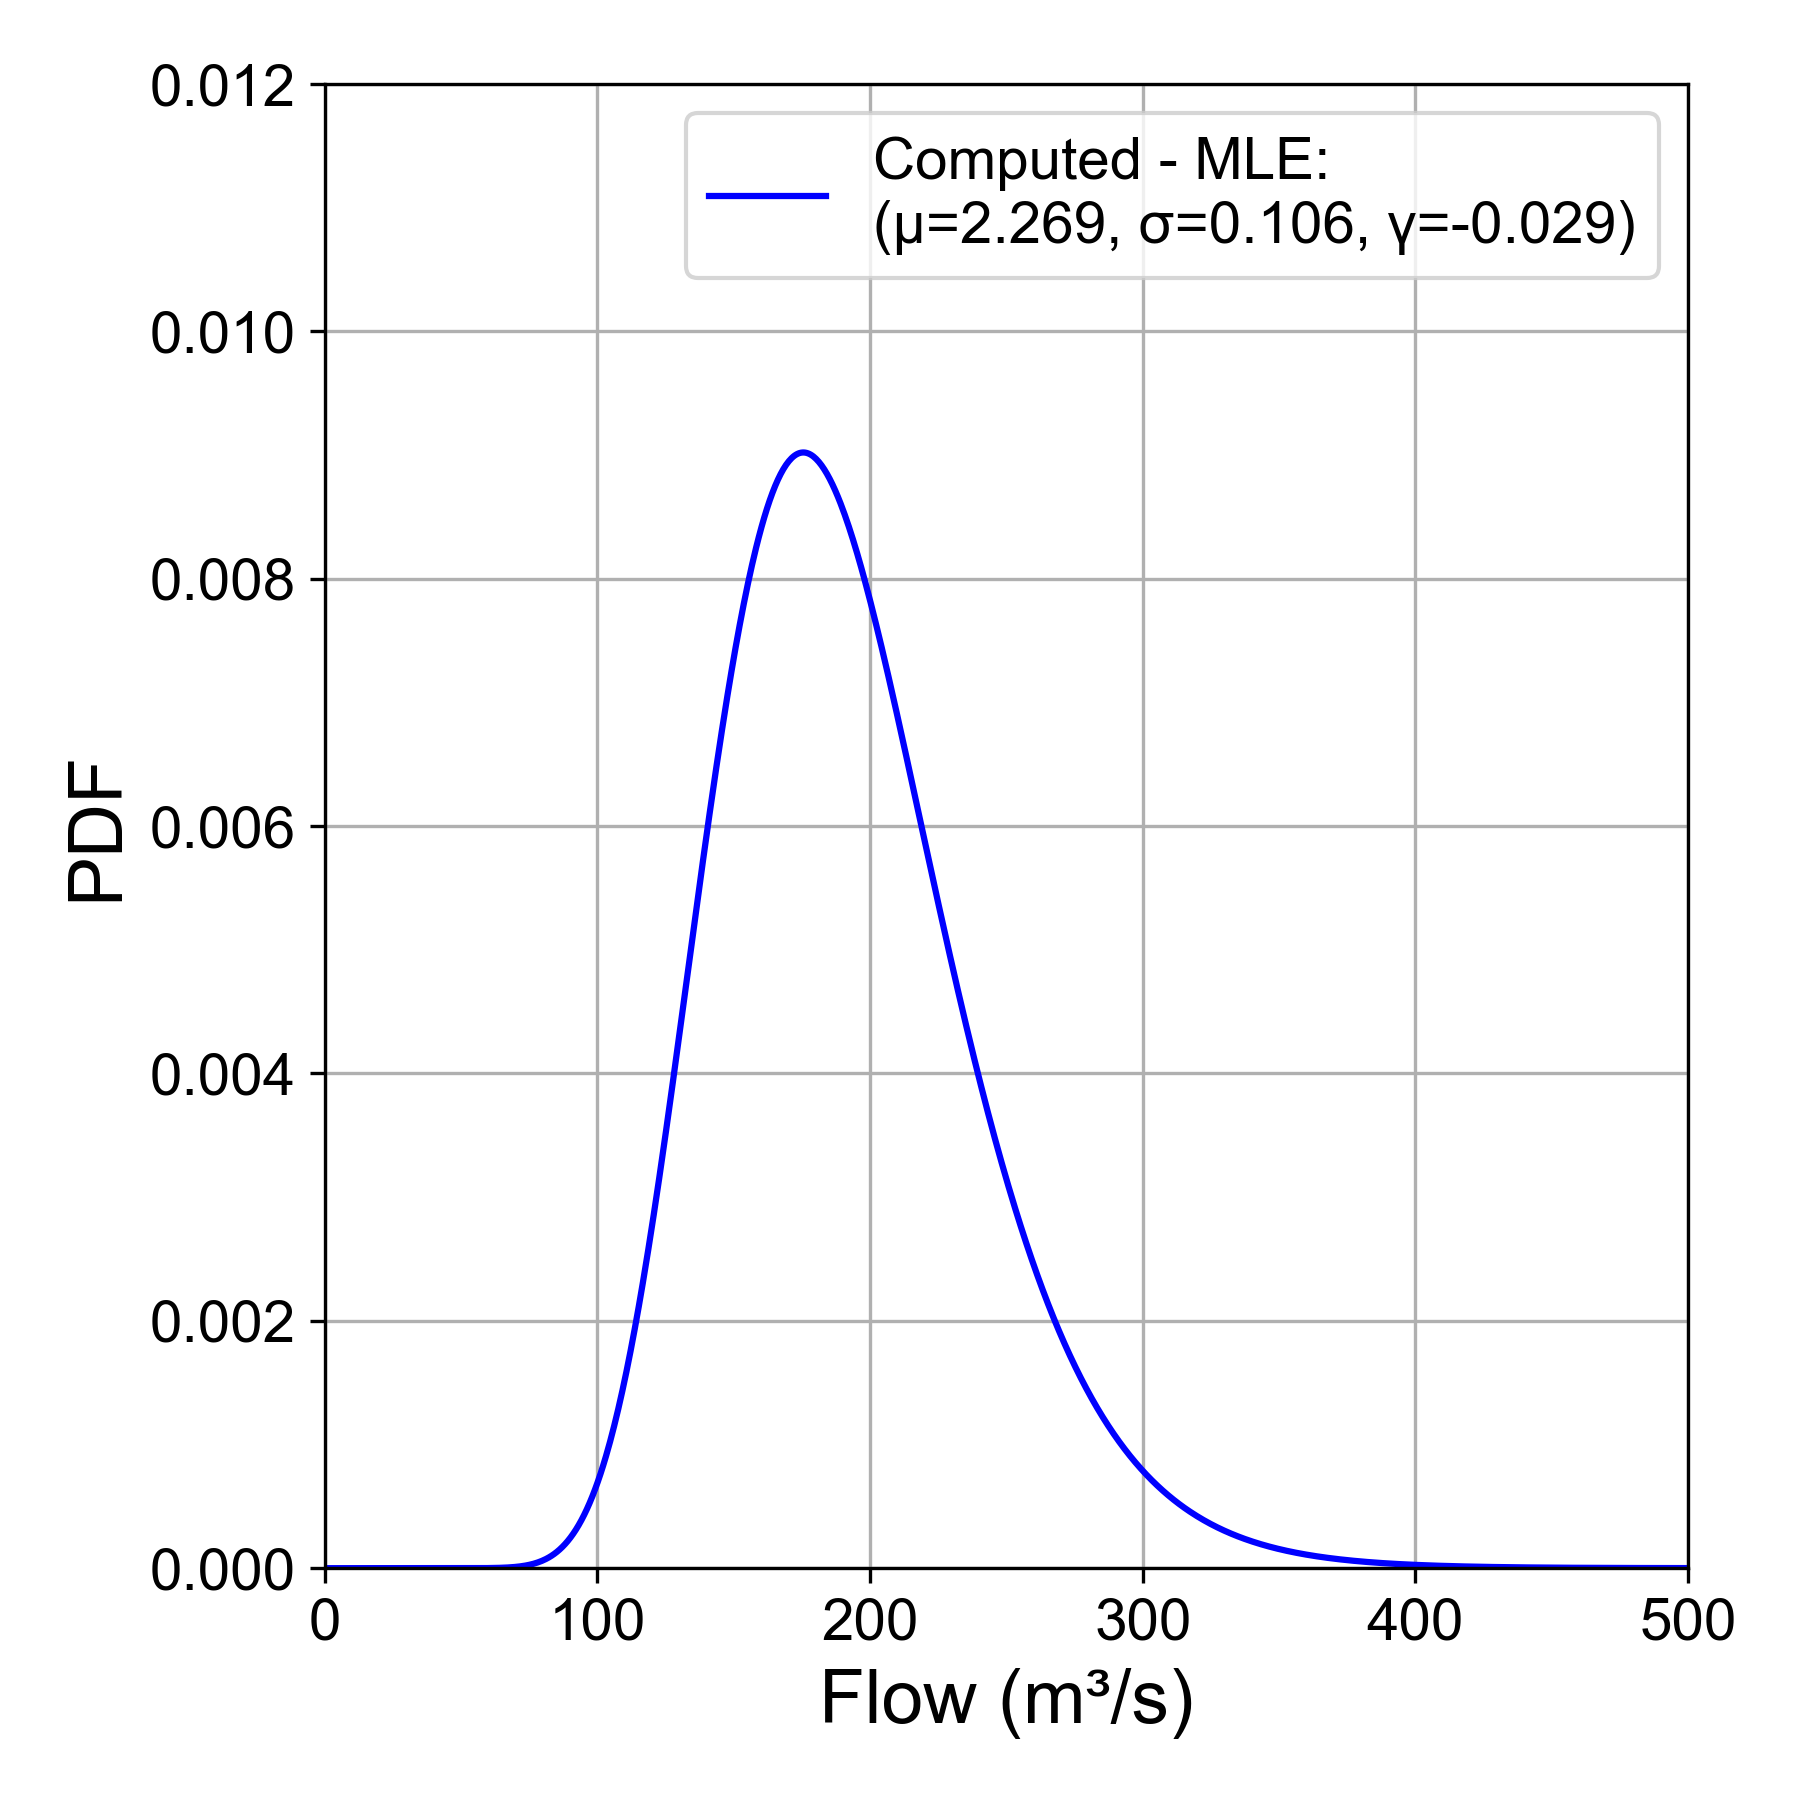
\includegraphics[width=1\linewidth]{_plots/HRA_LP3_MLE.png}
    \caption{LP3 distribution using the MLE method for the Harricana River dataset.}
    \label{fig:HRA_LP3_MLE}
\end{figure}

\begin{figure}[ht!]
    \centering
    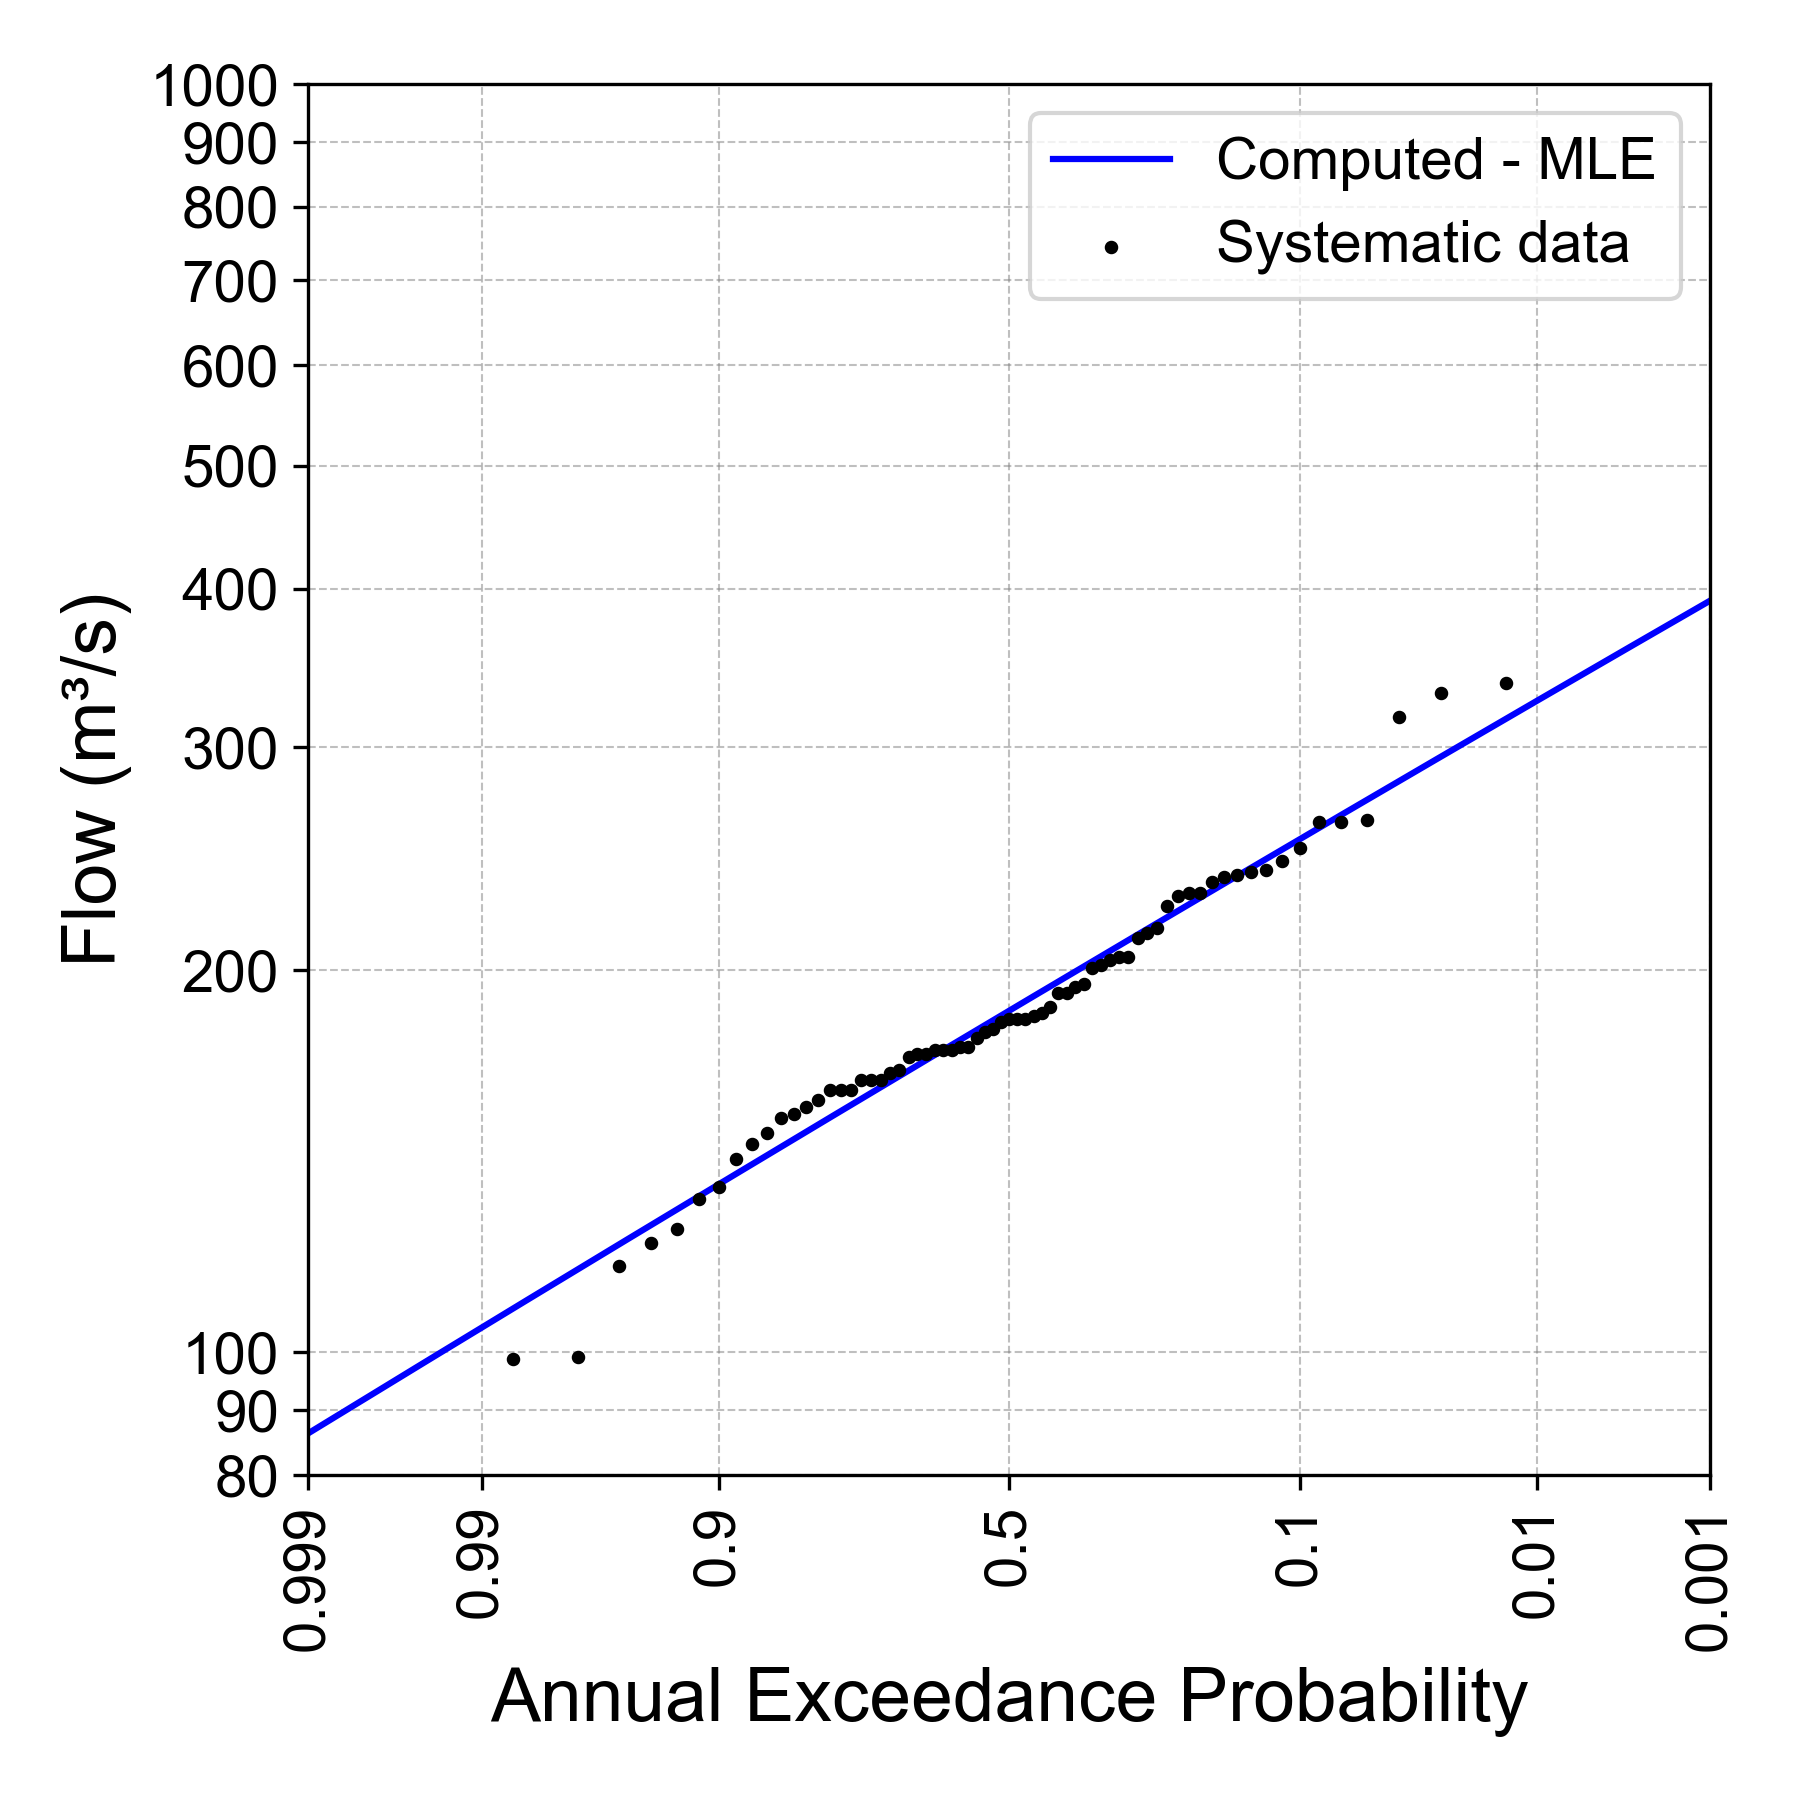
\includegraphics[width=1\linewidth]{_plots/HRA_flood_quantiles_MLE.png}
    \caption{Flood frequency curve using the MLE method for the Harricana River dataset.}
    \label{fig:HRA_flood_quantiles_MLE}
\end{figure}

The adaptive DE-MCzS algorithm demonstrates stable and efficient performance, with acceptance rates ranging from 0.525 to 0.533 across the five chains, as shown in Table \ref{table:HRA_acceptance}. Convergence diagnostics (Table \ref{table:HRA_Rhat}), indicate excellent chain convergence with $\hat{R}$ values near 1 for all parameters. The Effective Sample Size (ESS) is sufficiently high for $\mu$ and $\sigma$, although a lower ESS $\gamma$ suggests potential inefficiencies in sampling. Posterior marginal distributions and trace plots of $\mu, \sigma$ and $\gamma$ (Figure \ref{fig:HRA_posterior_combined_lp3}) further demonstrate stationary, well-mixed chains, and well-constrained parameter estimates, indicating an effective exploration of the posterior space.

\begin{figure*}[ht!]
    \centering
    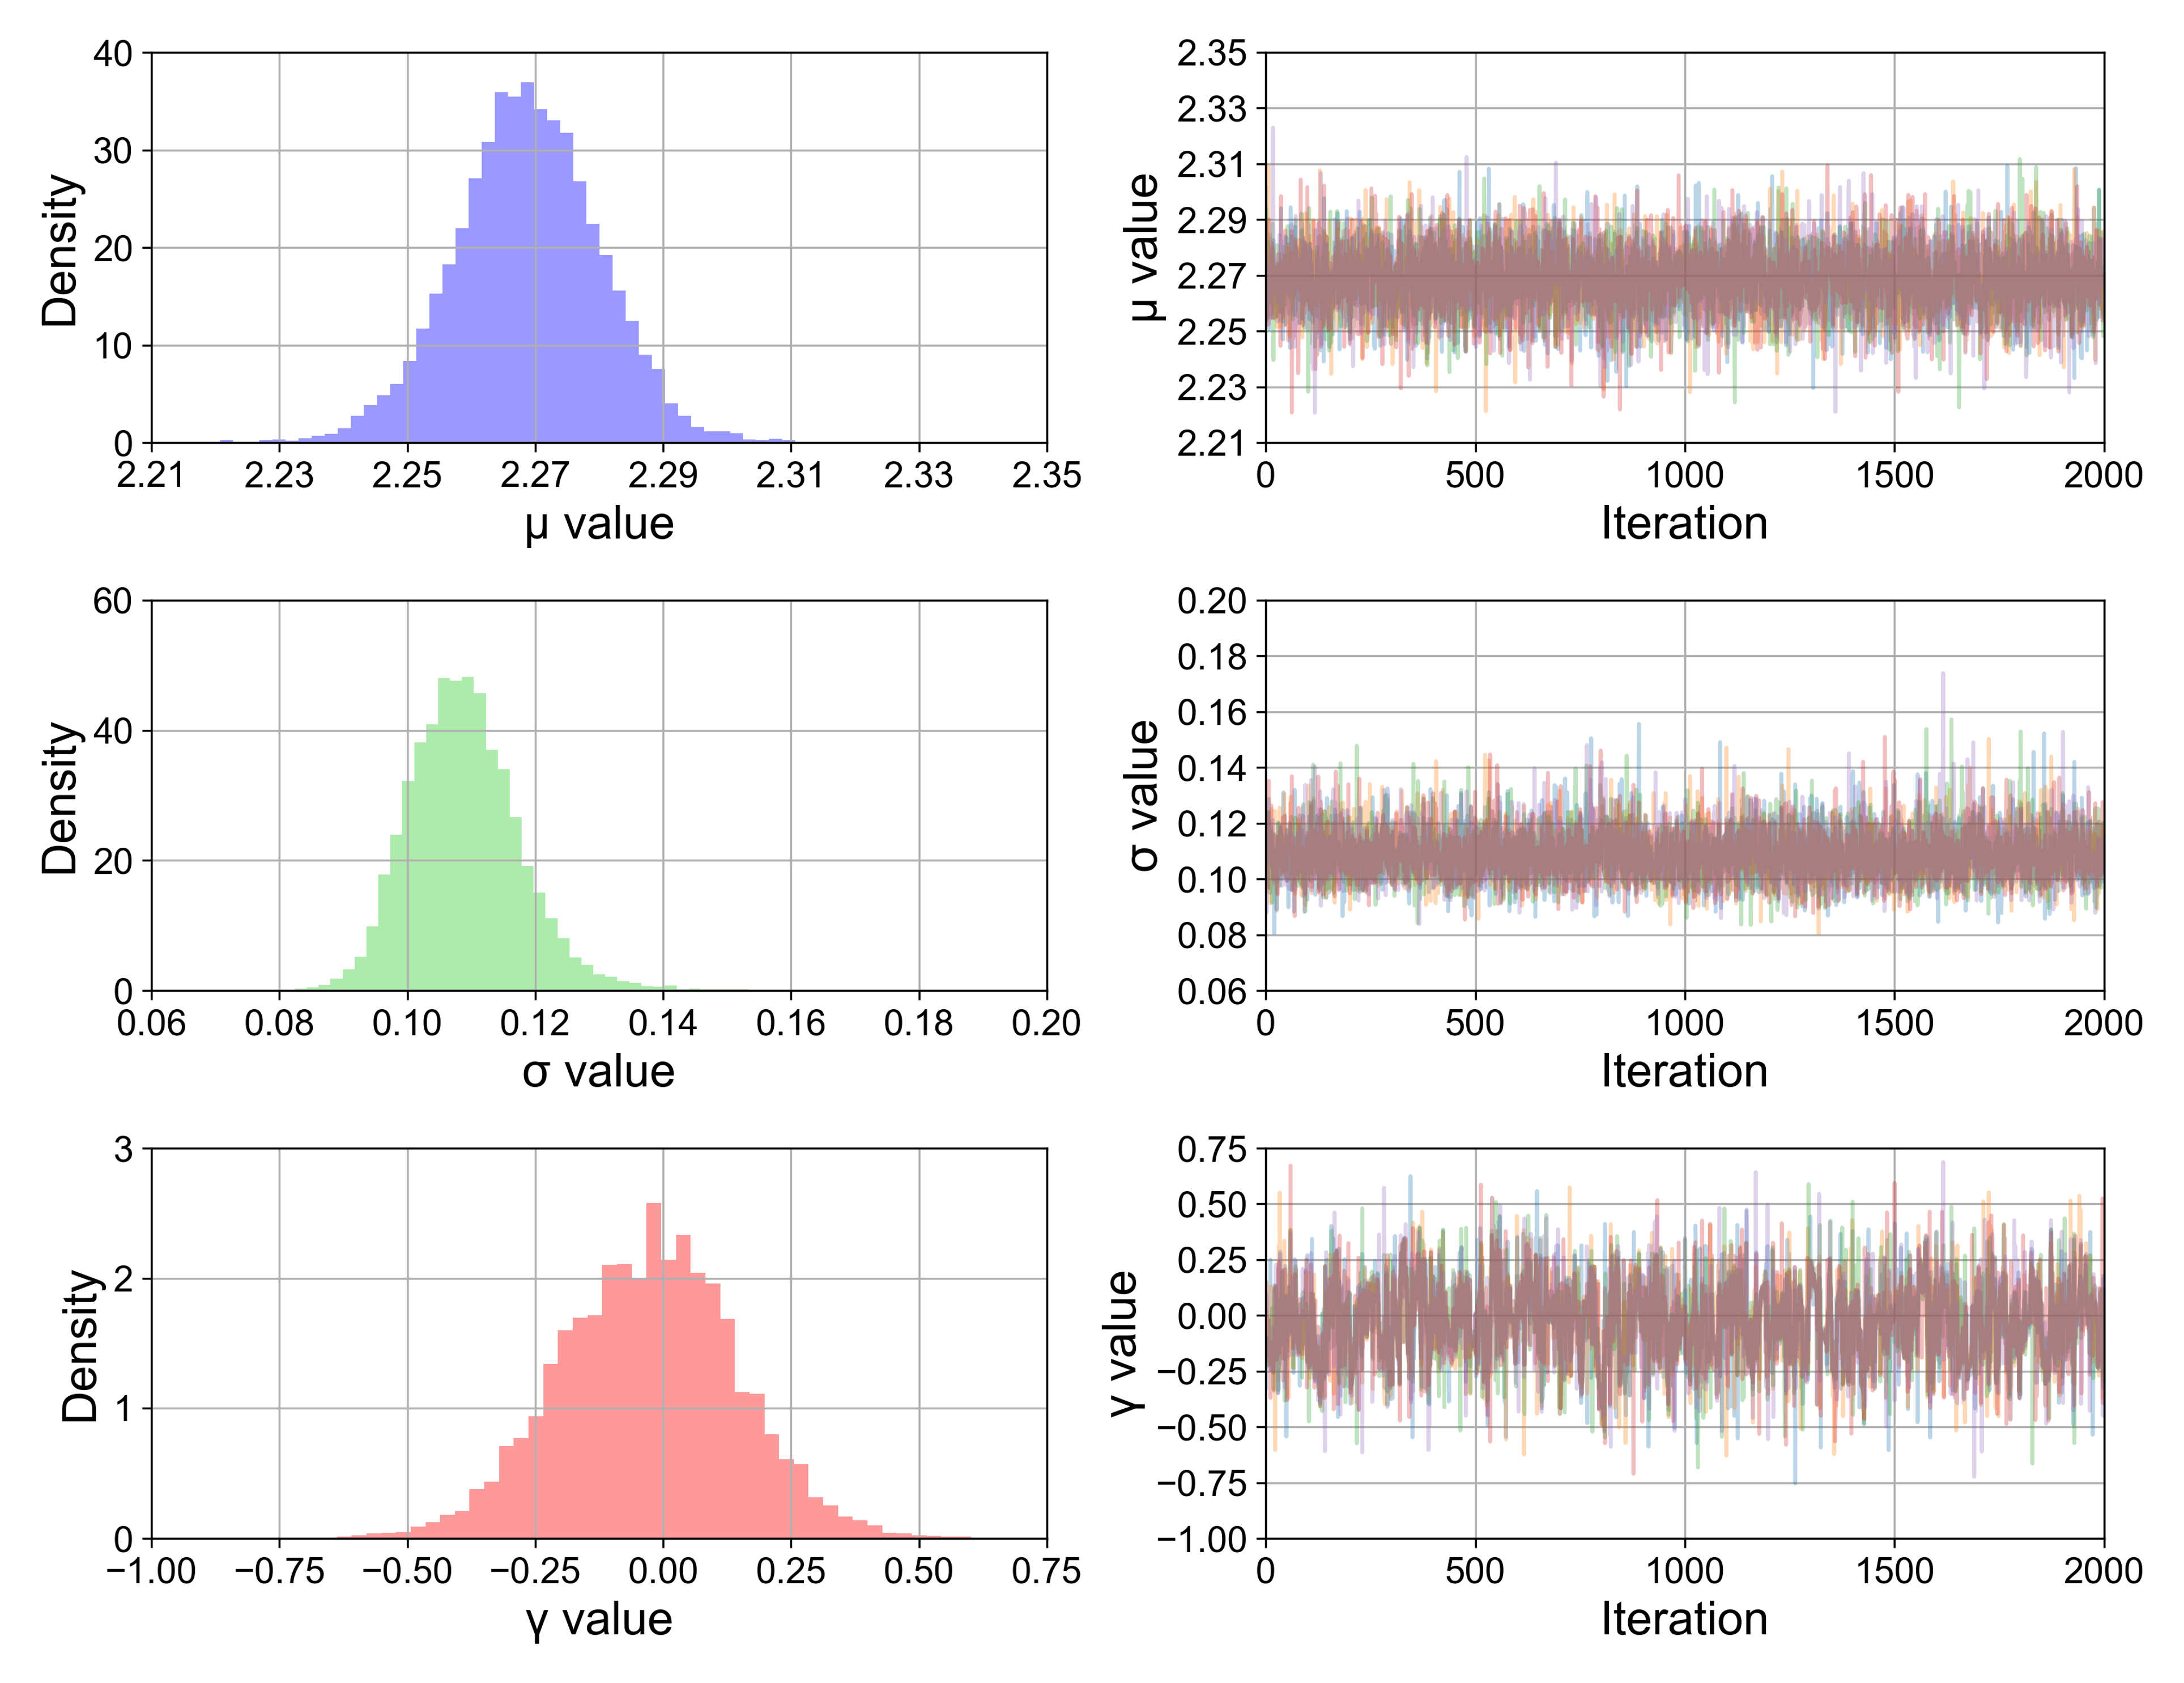
\includegraphics[width=1\linewidth]{_plots/HRA_posterior_combined_lp3.png}
    \caption{Posterior marginal distributions and trace plots for the $\mu$, $\sigma$, and $\gamma$ of LP3 distribution, derived from the Bayesian analysis of the Harricana River dataset. The trace plots checks convergence and efficient posterior sampling using the DE-MCzS algorithm.}
    \label{fig:HRA_posterior_combined_lp3}
\end{figure*}

\renewcommand{\arraystretch}{1.2}
% \begin{table}[H]
% \centering
% \caption{Acceptance rates for the DE-MCzS algorithm applied to the Harricana River dataset.}
% \begin{tabular}{l c c}
% \hline
% Chain No. & Number of Iterations & Acceptance Rate\\ \hline
% 1 & 2000 & 0.532 \\
% 2 & 2000 & 0.525 \\
% 3 & 2000 & 0.530 \\
% 4 & 2000 & 0.533 \\
% 5 & 2000 & 0.530 \\
% \hline
% \end{tabular}
% \label{table:HRA_acceptance}
% \end{table}

\renewcommand{\arraystretch}{1.2}
\begin{table}[H]
\centering
\caption{Acceptance rates for the DE-MCzS algorithm applied to the Harricana River dataset.}
\begin{tabular}{l c c c c c}
\hline
Chain No. &  1 & 2 & 3 & 4 & 5\\ \hline
Acceptance Rate & 0.532 & 0525 & 0.530 & 0.533 & 0.530\\
Iterations & 2000 & 2000 & 2000 & 2000 &2000 \\
\hline
\end{tabular}
\label{table:HRA_acceptance}
\end{table}

\renewcommand{\arraystretch}{1.2}
\begin{table}[H]
\centering
\caption{Comparison of convergence diagnostics between Computed and BestFit results for the LP3 parameters estimated using the Harricana River dataset.}
\begin{tabular}{l c c c c}
\hline
 & \multicolumn{2}{c}{$\hat{R}$} & \multicolumn{2}{c}{ESS} \\ 
Parameter & Computed & BestFit & Computed & BestFit \\ \hline
$\mu$ & 0.9998 & 1.000 & 8,571 & 10,000 \\
$\sigma$ & 1.0000 & 1.000 & 8,950 & 9,372 \\
$\gamma$ & 1.0001 & 1.000 & 2,204 & 10,000 \\
\hline
\end{tabular}
\label{table:HRA_Rhat}
\end{table}

\begin{figure}[H]
    \centering
    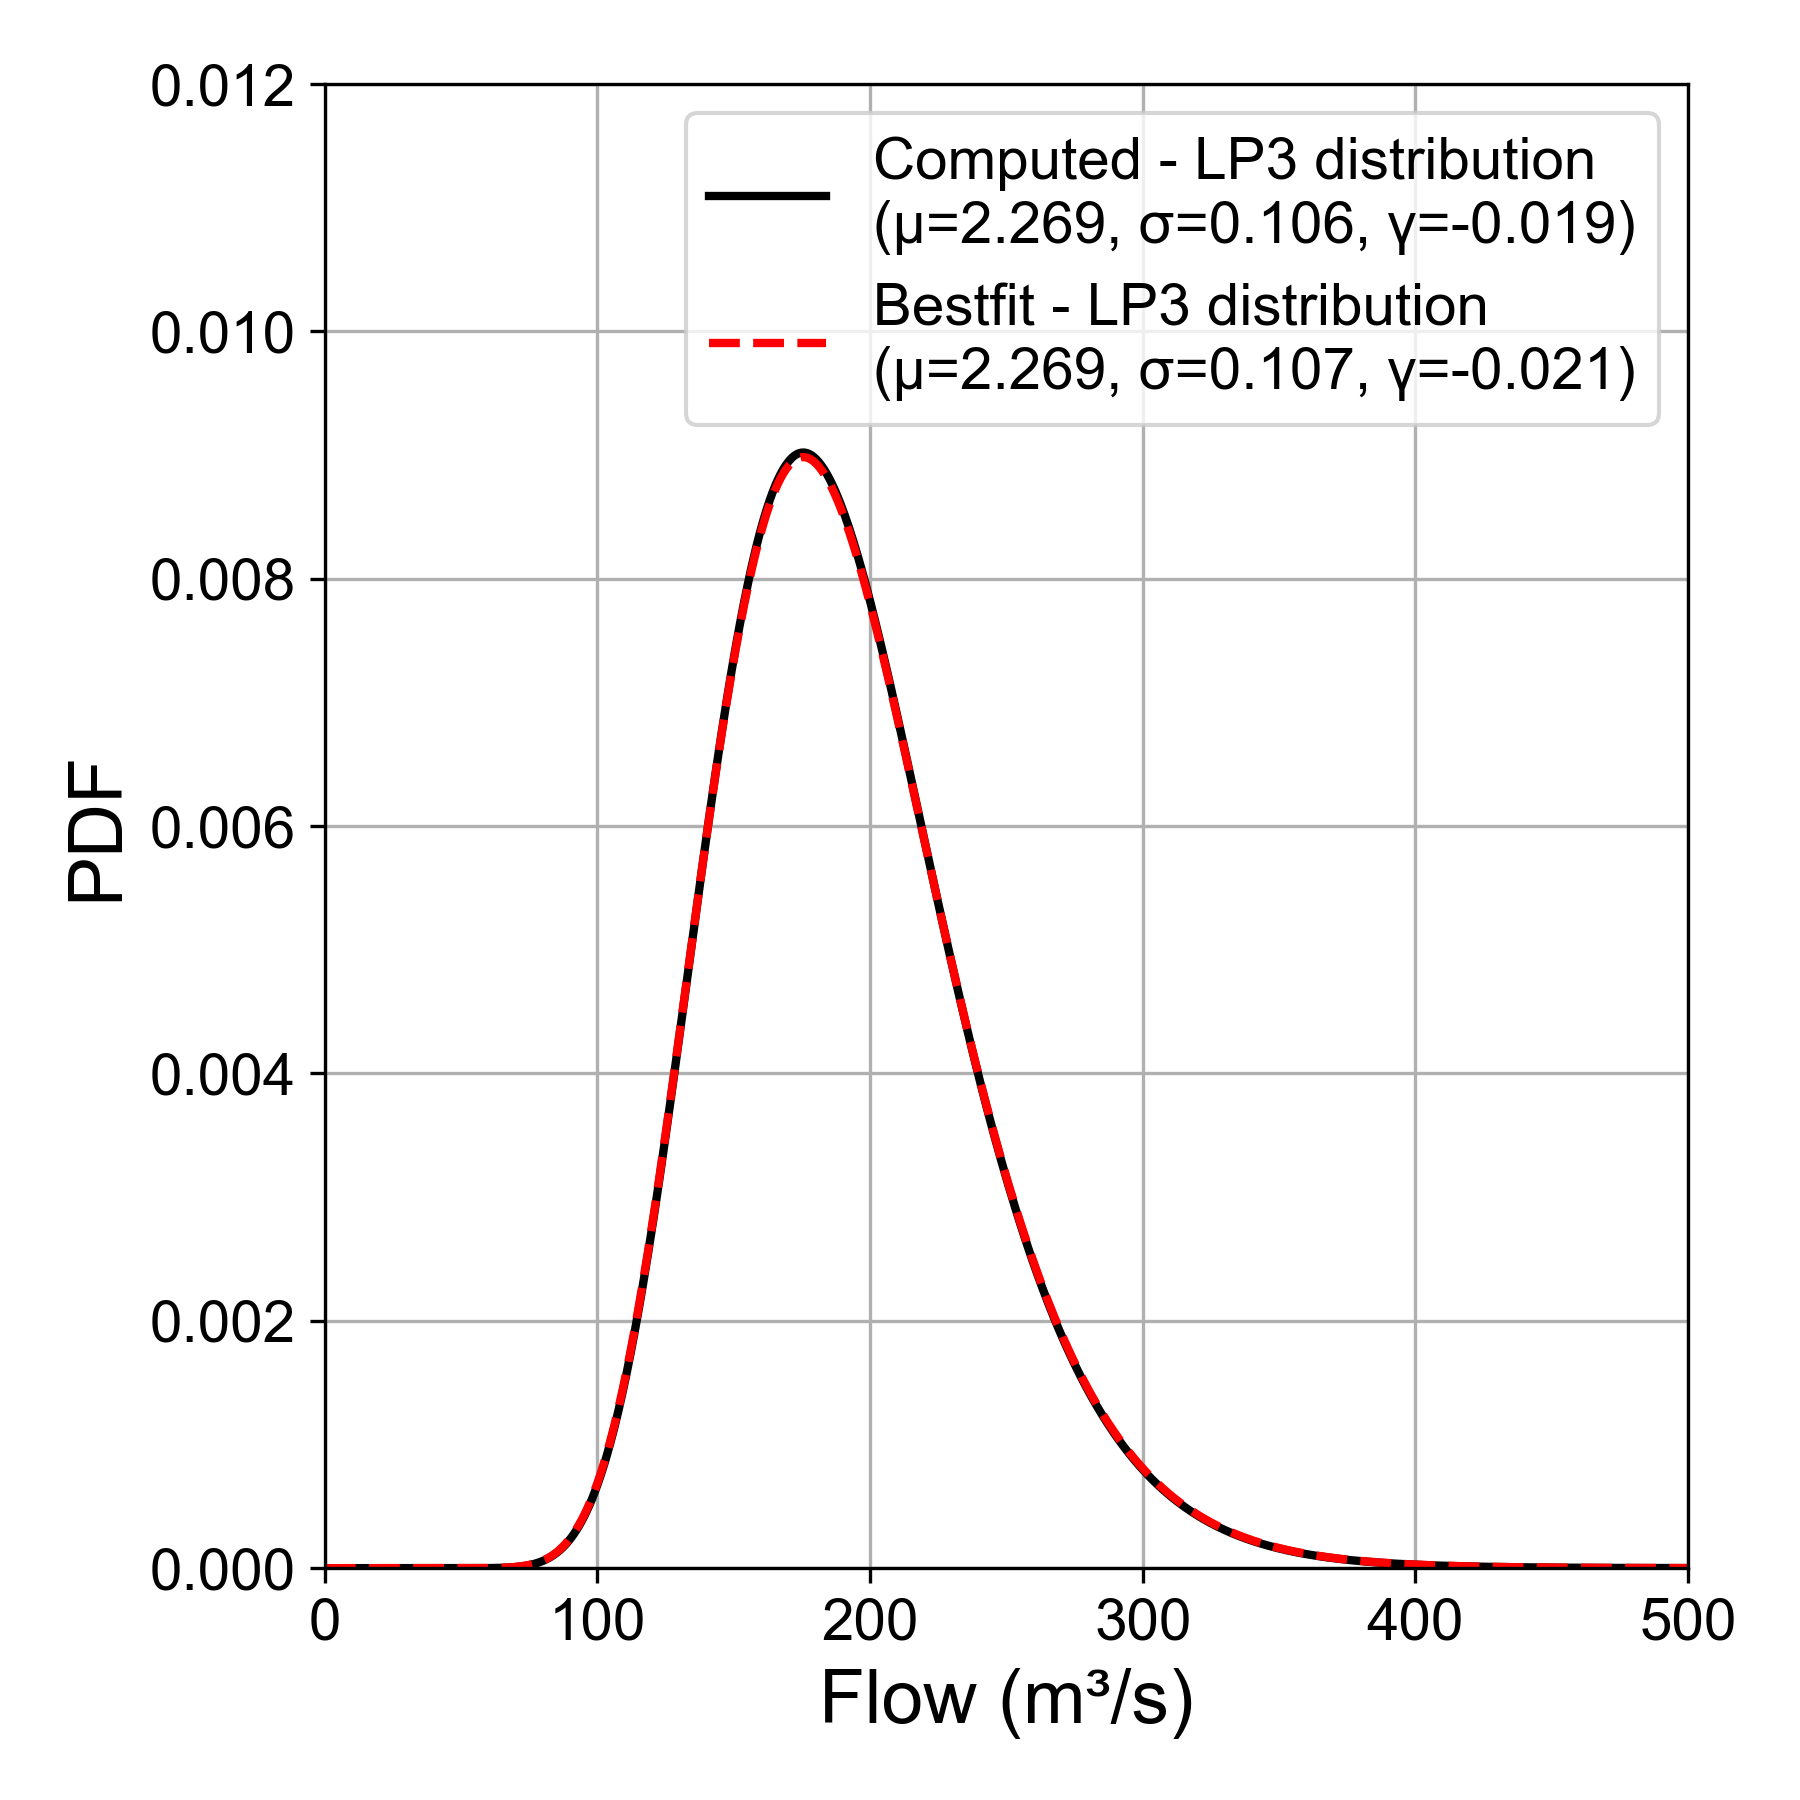
\includegraphics[width=1\linewidth]{_plots/HRA_LP3_comparison.png}
    \caption{Comparison of the posterior mode LP3 distribution with the BestFit results for the Harricana River dataset. }
    \label{fig:HRA_LP3_comparison}
\end{figure}

In verification, the computed LP3 distribution at the posterior mode (Figure \ref{fig:HRA_LP3_comparison}) aligns exceptionally well with the results obtained from BestFit results. With the same noise term applied (labeled as noise testing), we were able to reproduce the posterior predictive distributions and their 90\% credible intervals on the flood frequency curve (Figure \ref{fig:HRA_bayesian_flood_quantiles_lp3}). Overall, an excellent consistency was achieved with BestFit. Minor discrepancies at the distribution tails likely result from differences in the random seed generation.

\begin{figure*}[ht!]
    \centering
    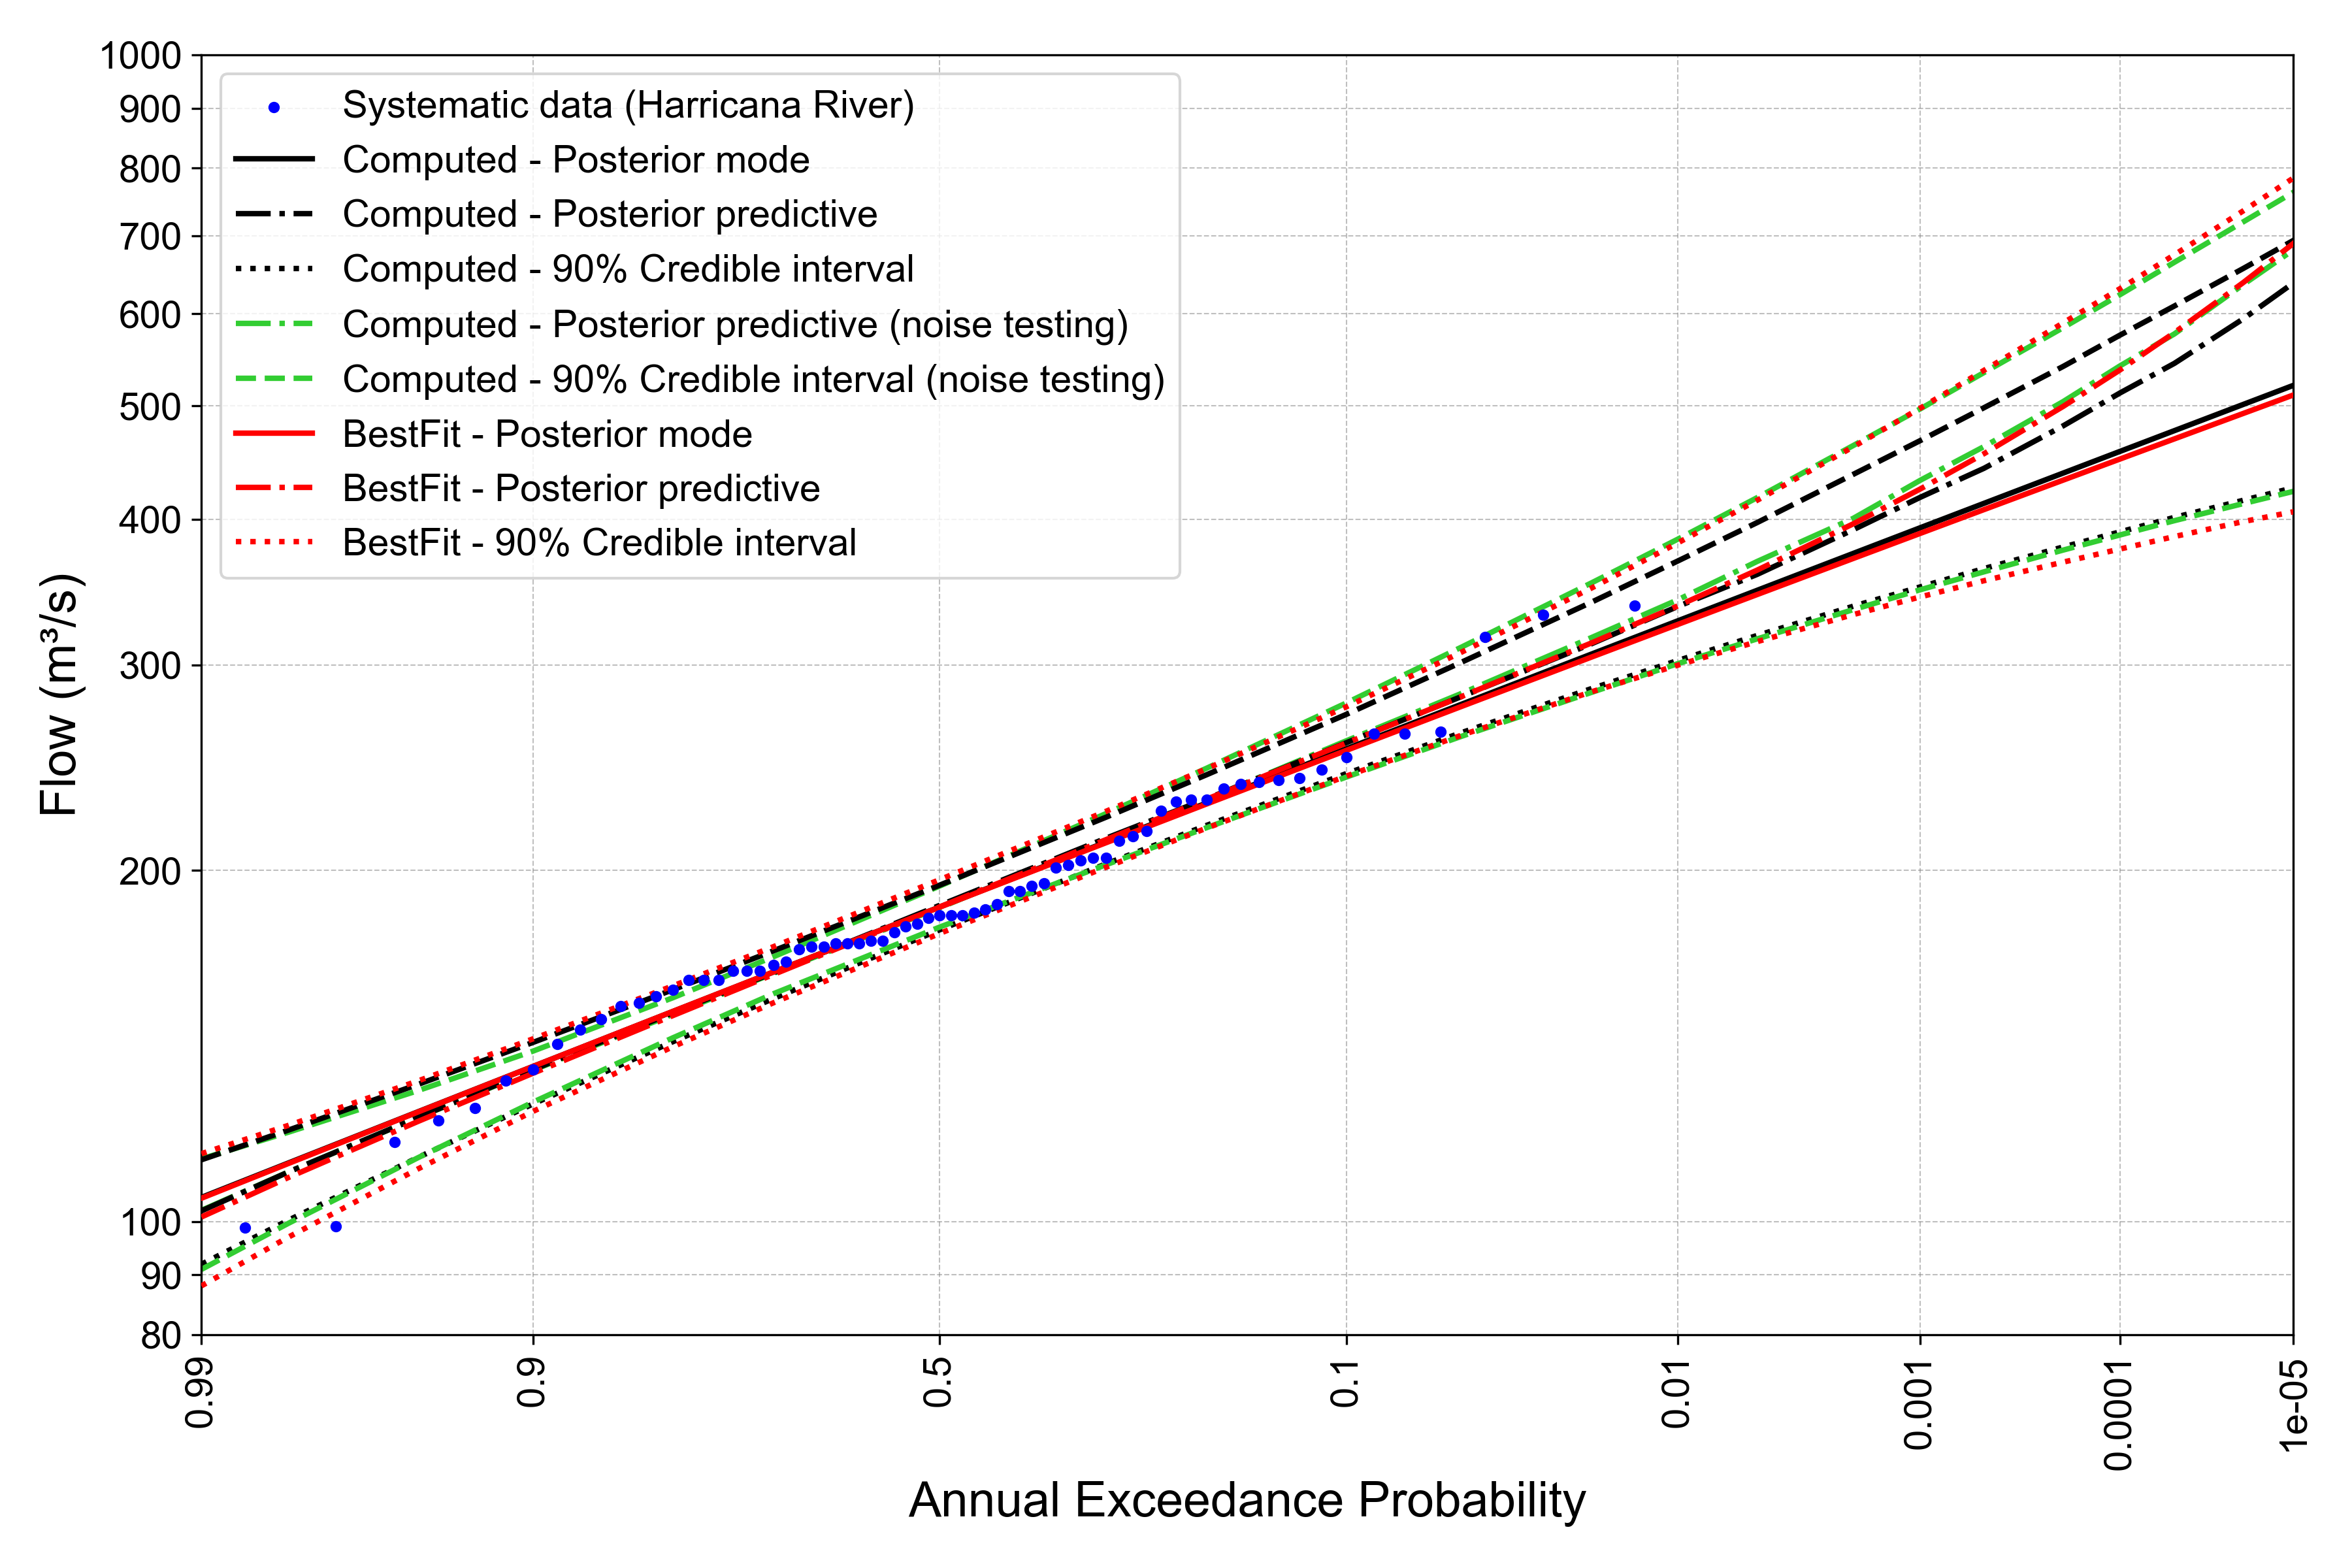
\includegraphics[width=1\linewidth]{_plots/HRA_bayesian_flood_quantiles_lp3.png}
    \caption{Comparison of Bayesian flood frequency curves with BestFit for the Harricana River dataset. Noise testing refers to the use of the same perturbation term as employed in BestFit to ensure consistency in model comparisons.}
    \label{fig:HRA_bayesian_flood_quantiles_lp3}
\end{figure*}

\subsection{Case study 2: O.C. Fisher Dam, USA}

The second case study examines both stationary FFA and NSFFA for the O.C. Fisher Dam dataset. The stationary FFA assumes constant parameters over time with uniform priors: 
\begin{align*}
    Y \mid \mu, \sigma, \gamma &\sim \text{LP3}(\mu, \sigma, \gamma)\\
    \mu &\sim \text{Uniform}(0,3)\\
    \sigma &\sim \text{Uniform}(0,2)\\
    \gamma &\sim \text{Uniform}(-2,2)
\end{align*}

The NSFFA models incorporate time-dependent trends for the location parameter ($\mu$), while $\sigma$ and $\gamma$ have the same prior as the stationary FFA model:
\begin{align*}
    Y \mid \mu_t, \sigma, \gamma &\sim \text{LP3}(\mu_t, \sigma, \gamma)\\
    \mu_t &=\beta_0 + \beta_1 \cdot t \quad \text{(linear)}\\
    \mu_t &=\beta_0 \cdot \exp(\beta_1 \cdot t ) \quad \text{ (exponential)}\\
    \beta_0 &\sim \text{Uniform}(0,3)\\
    \beta_1 &\sim \text{Uniform}(-1,1)
\end{align*}


\begin{figure}[H]
    \centering
    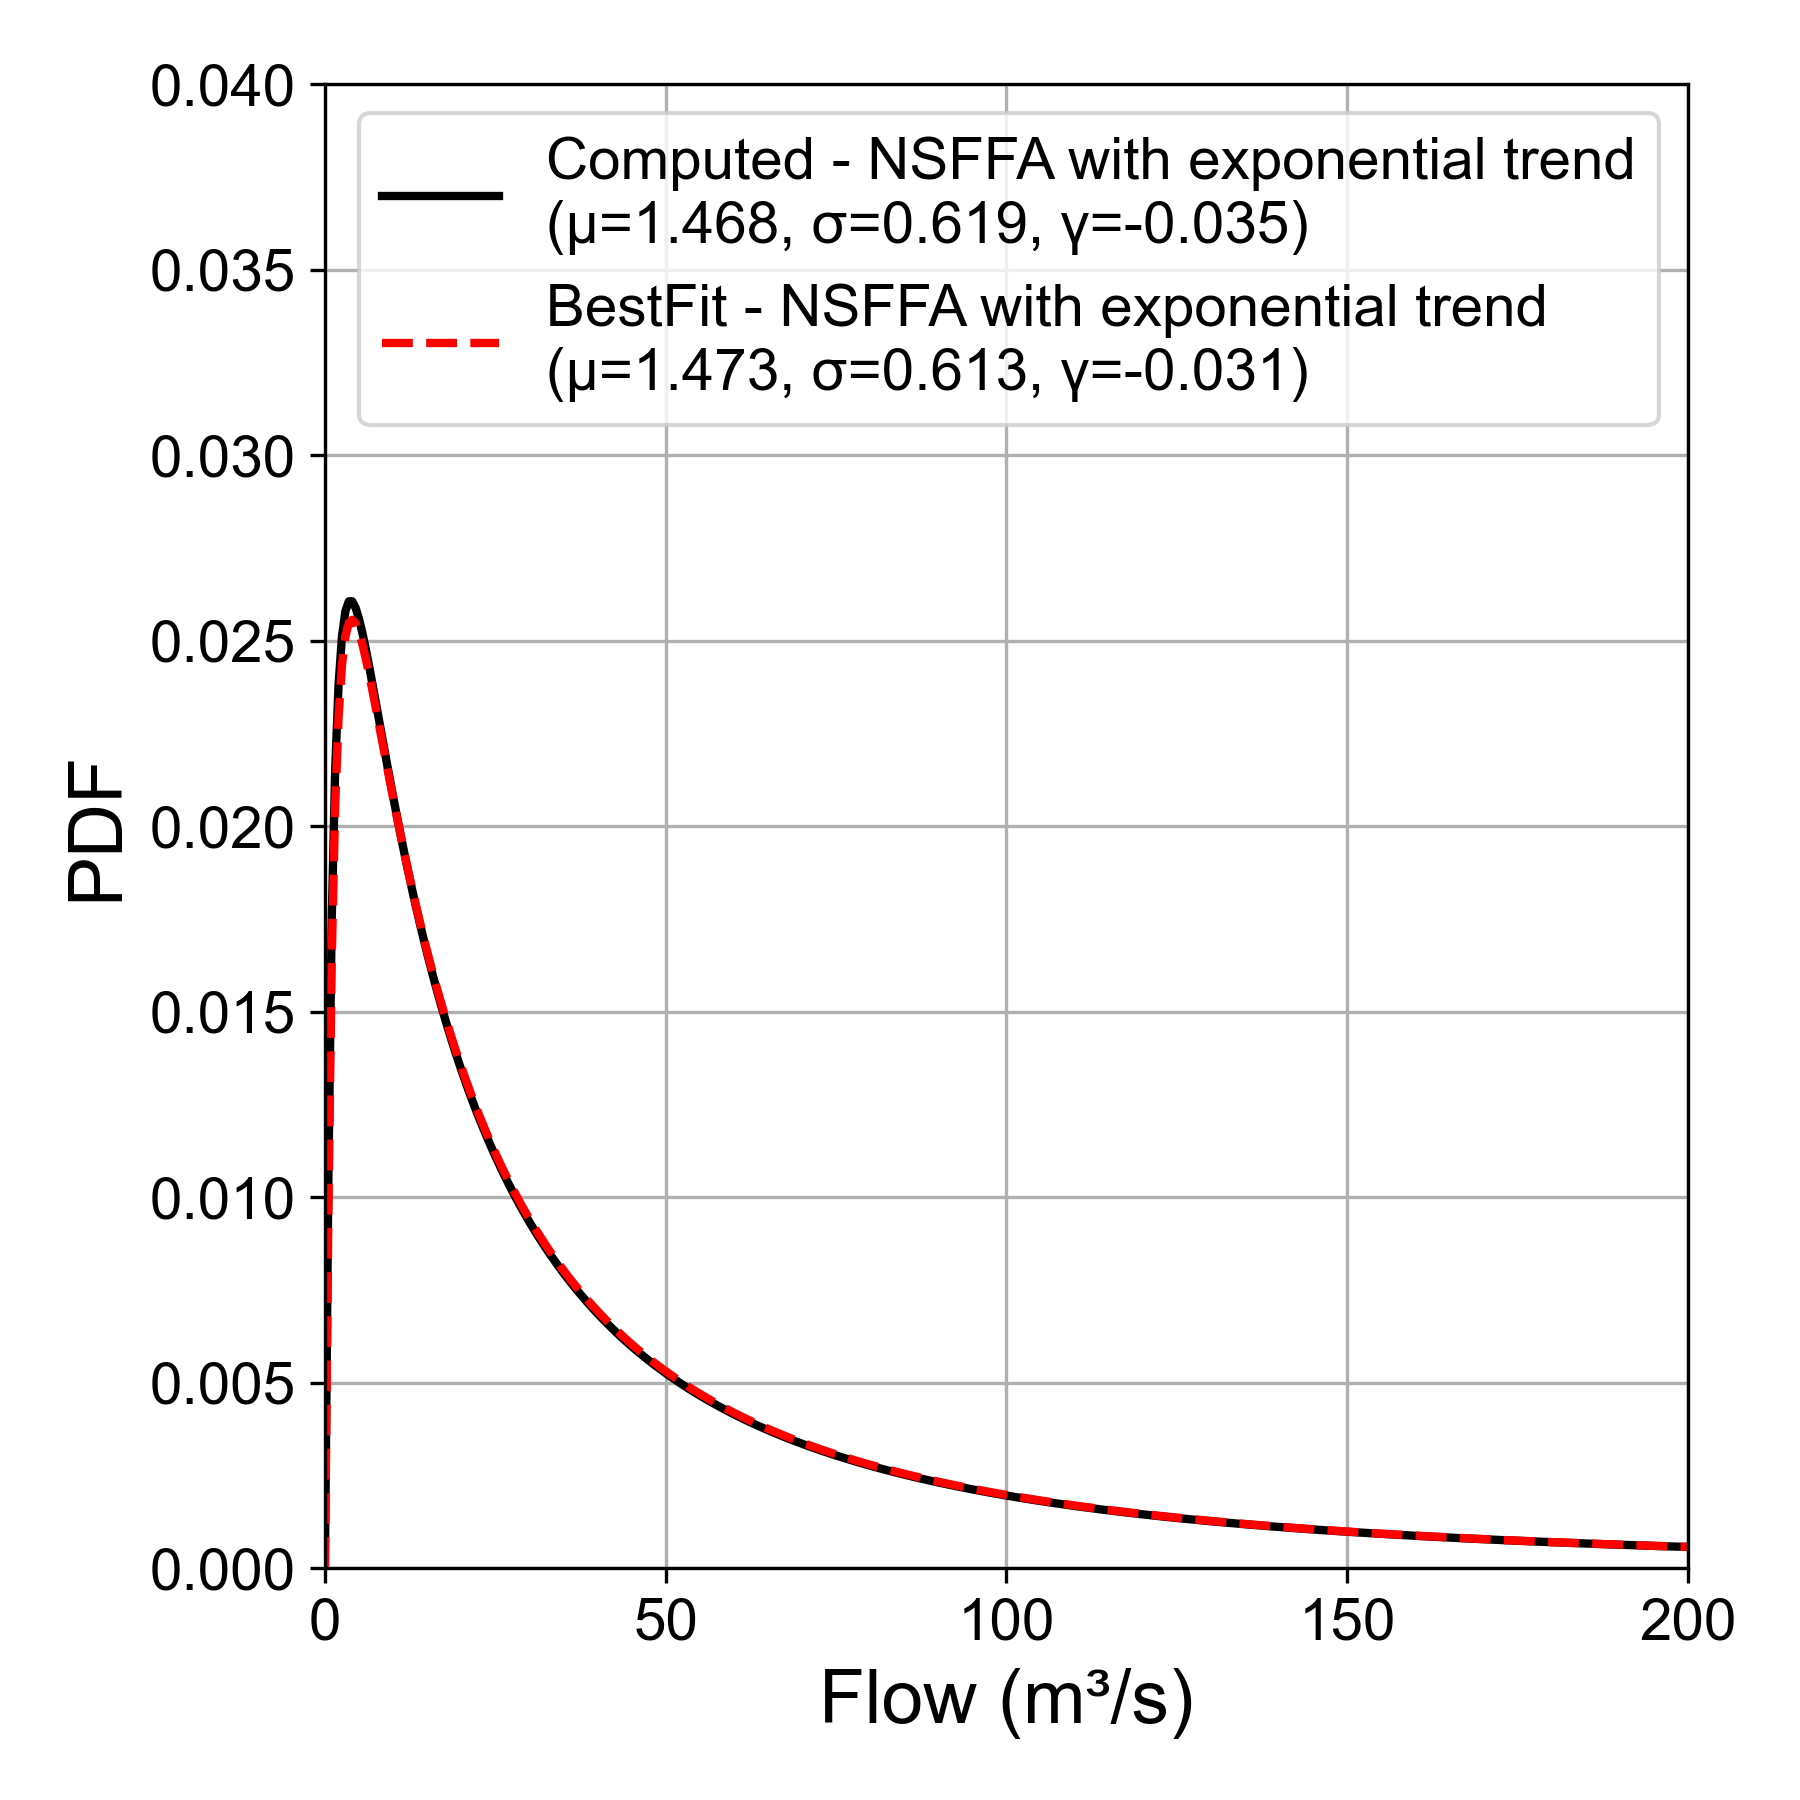
\includegraphics[width=1\linewidth]{_plots/OCD_LP3_exponential_mu_comparison.png}
    \caption{Comparison of the posterior mode LP3 distribution with the BestFit results under the linear trend NSFFA model for the Fisher Dam dataset.}
    \label{fig:OCD_LP3_exponential_mu_comparison}
\end{figure}

The posterior mode estimates for the three models — stationary FFA, NSFFA with a linear trend, and NSFFA with an exponential trend - were benchmarked against the results from BestFit (Table \ref{table:OCD_comparison_computed_bestfit}). Overall, the computed parameters demonstrate a strong agreement with BestFit results. The exponential trend model shows notable deviations in parameters $\beta_1$ and $\gamma$. However, the LP3 distribution derived from the this model (Figure \ref{fig:OCD_LP3_exponential_mu_comparison}) closely aligns with BestFit. Performance evaluation of the adaptive DE-MCzS algorithm and verification of flood frequency curves are presented in Appendix C. The discrepancies observed in the posterior predictive distributions and credible intervals can be attributed to variations in the noise term as shown in Figure \ref{fig:HRA_bayesian_flood_quantiles_lp3}.

\renewcommand{\arraystretch}{1.2}
\begin{table*}
\centering
\caption{Comparison of computed and BestFit posterior mode estimates for different models, including FFA, NSFFA (TI of 1949) with linear and exponential trends, using the Fisher Dam dataset.}
\begin{tabular}{llccc}
\hline
Model & Parameter & Computed & BestFit & \textbf{\% Difference} \\ \hline
Stationary FFA & $\mu$ & 1.303 & 1.300 & 0.17\% \\
& $\sigma$ & 0.699 & 0.696 & 0.50\% \\
& $\gamma$ & 0.178 & 0.178 & 0.11\% \\ \hline
NSFFA with linear trend & $\beta_0$ & 1.869 & 1.871 & -0.15\% \\
& $\beta_1$ & -0.0108 & -0.0109 & -1.12\% \\
& $\sigma$ & 0.614 & 0.613 & 0.21\% \\
& $\gamma$ & -0.048 & -0.047 & 1.44\% \\ \hline
NSFFA with exponential trend & $\beta_0$ & 1.934 & 1.871 & 3.37\% \\
& $\beta_1$ & -0.00811 & -0.01091 & -25.62\% \\
& $\sigma$ & 0.619 & 0.613 & 1.01\% \\
& $\gamma$ & -0.0345 & -0.0469 & -26.49\% \\ \hline
\end{tabular}
\label{table:OCD_comparison_computed_bestfit}
\end{table*}

\begin{figure}[H]
    \centering
    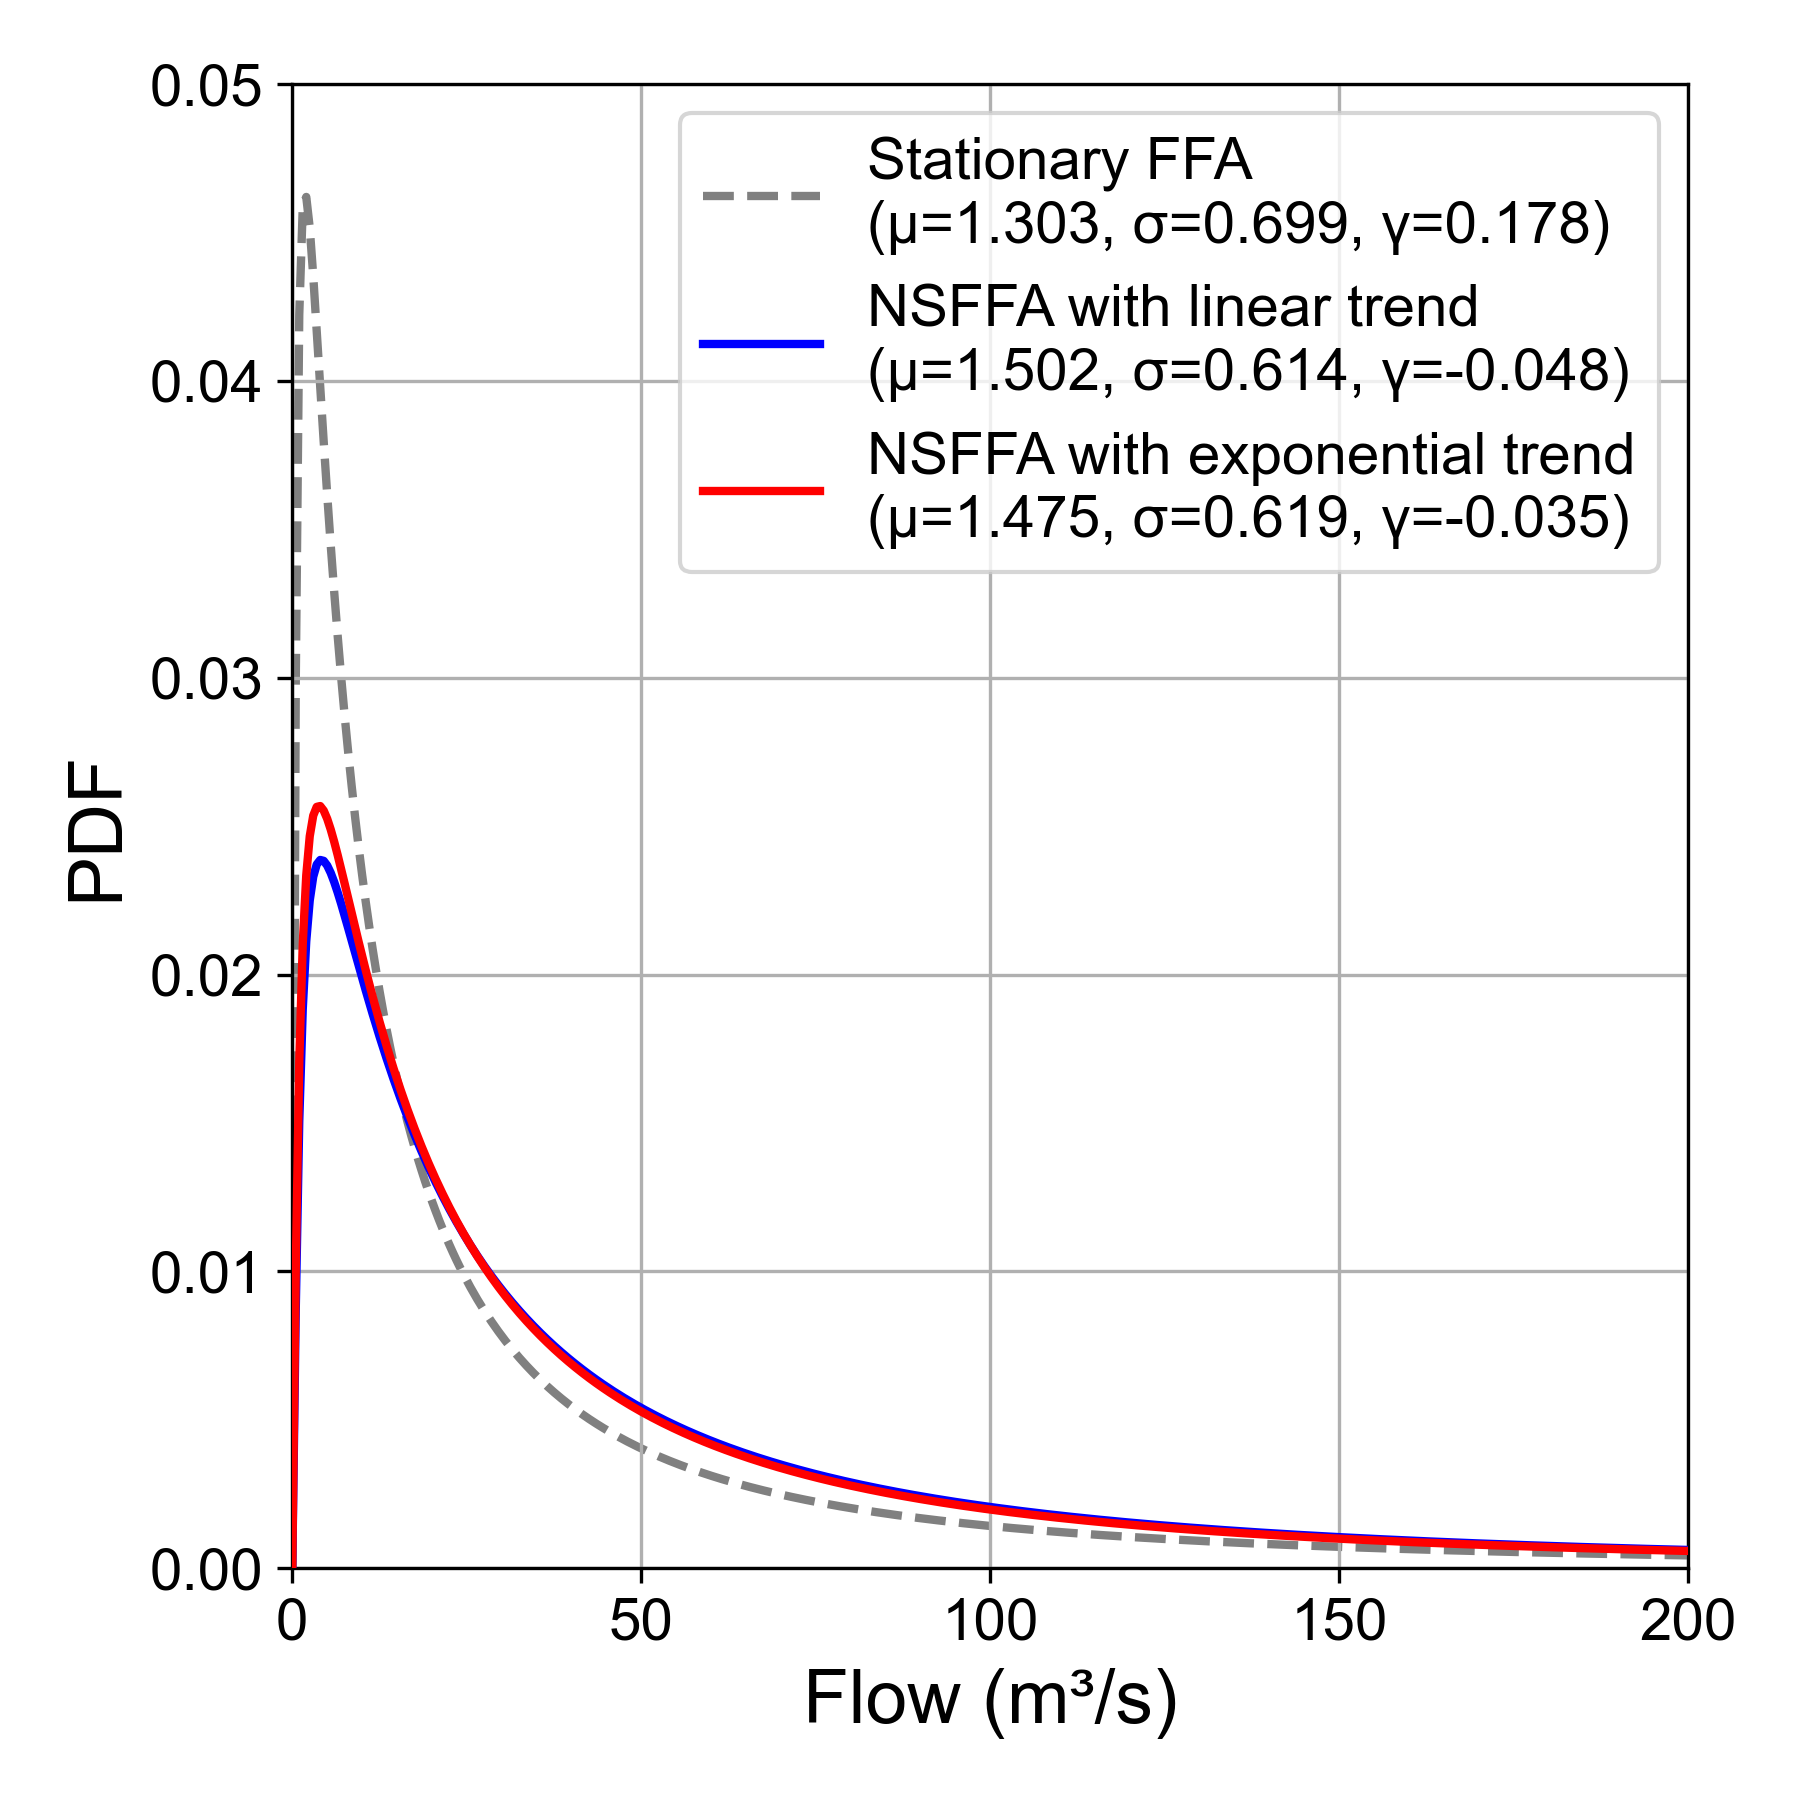
\includegraphics[width=1\linewidth]{_plots/OCD_LP3_nonstationary_comparison.png}
    \caption{Comparison of posterior mode LP3 distribution for FFA and NSFFA using the Fisher Dam dataset, with the middle year (1949) selected as the time index for analysis.}
    \label{fig:OCD_LP3_nonstationary_comparison}
\end{figure}

The LP3 distributions, shown in Figure \ref{fig:OCD_LP3_nonstationary_comparison}, were analyzed with the middle year (1949) selected as the time index for NSFFA. The stationary FFA model exhibits a higher peak density, reflecting concentrated probabilities near the central tendency, while the NSFFA models (both linear and exponential trends) show reduced peak densities and heavier tails, indicating greater uncertainty. These differences are further reflected in flood frequency curves (Figure \ref{fig:OCD_bayesian_flood_quantiles_lp3_linear_mu_TI}). The stationary FFA model aligns closely with observed data, particularly for frequent AEPs. In contrast, the NSFFA curves are generally flatter, predicting higher flows for frequent events but significantly lower flows for extreme events. Between the linear and exponential trend NSFFA models, the resulting distributions are broadly similar, with minor differences in peak density. This suggests that the choice of trend type has a negligible effect on the flood frequency curves for the Fisher Dam dataset.

Figure \ref{fig:OCD_LP3_linear_mu_comparison_TI} explores the impact of time index selection on LP3 distributions under the linear trend model. Earlier time indices, such as 1919 ($\mu = 1.825$), correspond to higher mean flow values and exhibit lower peak densities and higher variance. As the time index advances toward future years (e.g., 2049, $\mu = 0.423$), the distribution become narrower with higher peak densities and lower variance. This indicates a systematic reduction in mean flows and increased concentration of probabilities around smaller values. The impact of time index selection on flood frequency curves is illustrated in Figure \ref{fig:OCD_bayesian_flood_quantiles_lp3_linear_mu_TI} under the same model. Earlier TIs (e.g., 1919) predict higher flow values, while later TIs (e.g., 2049) yield lower flow values, which aligns with the observed decline in mean flow over time.

\begin{figure}[H]
    \centering
    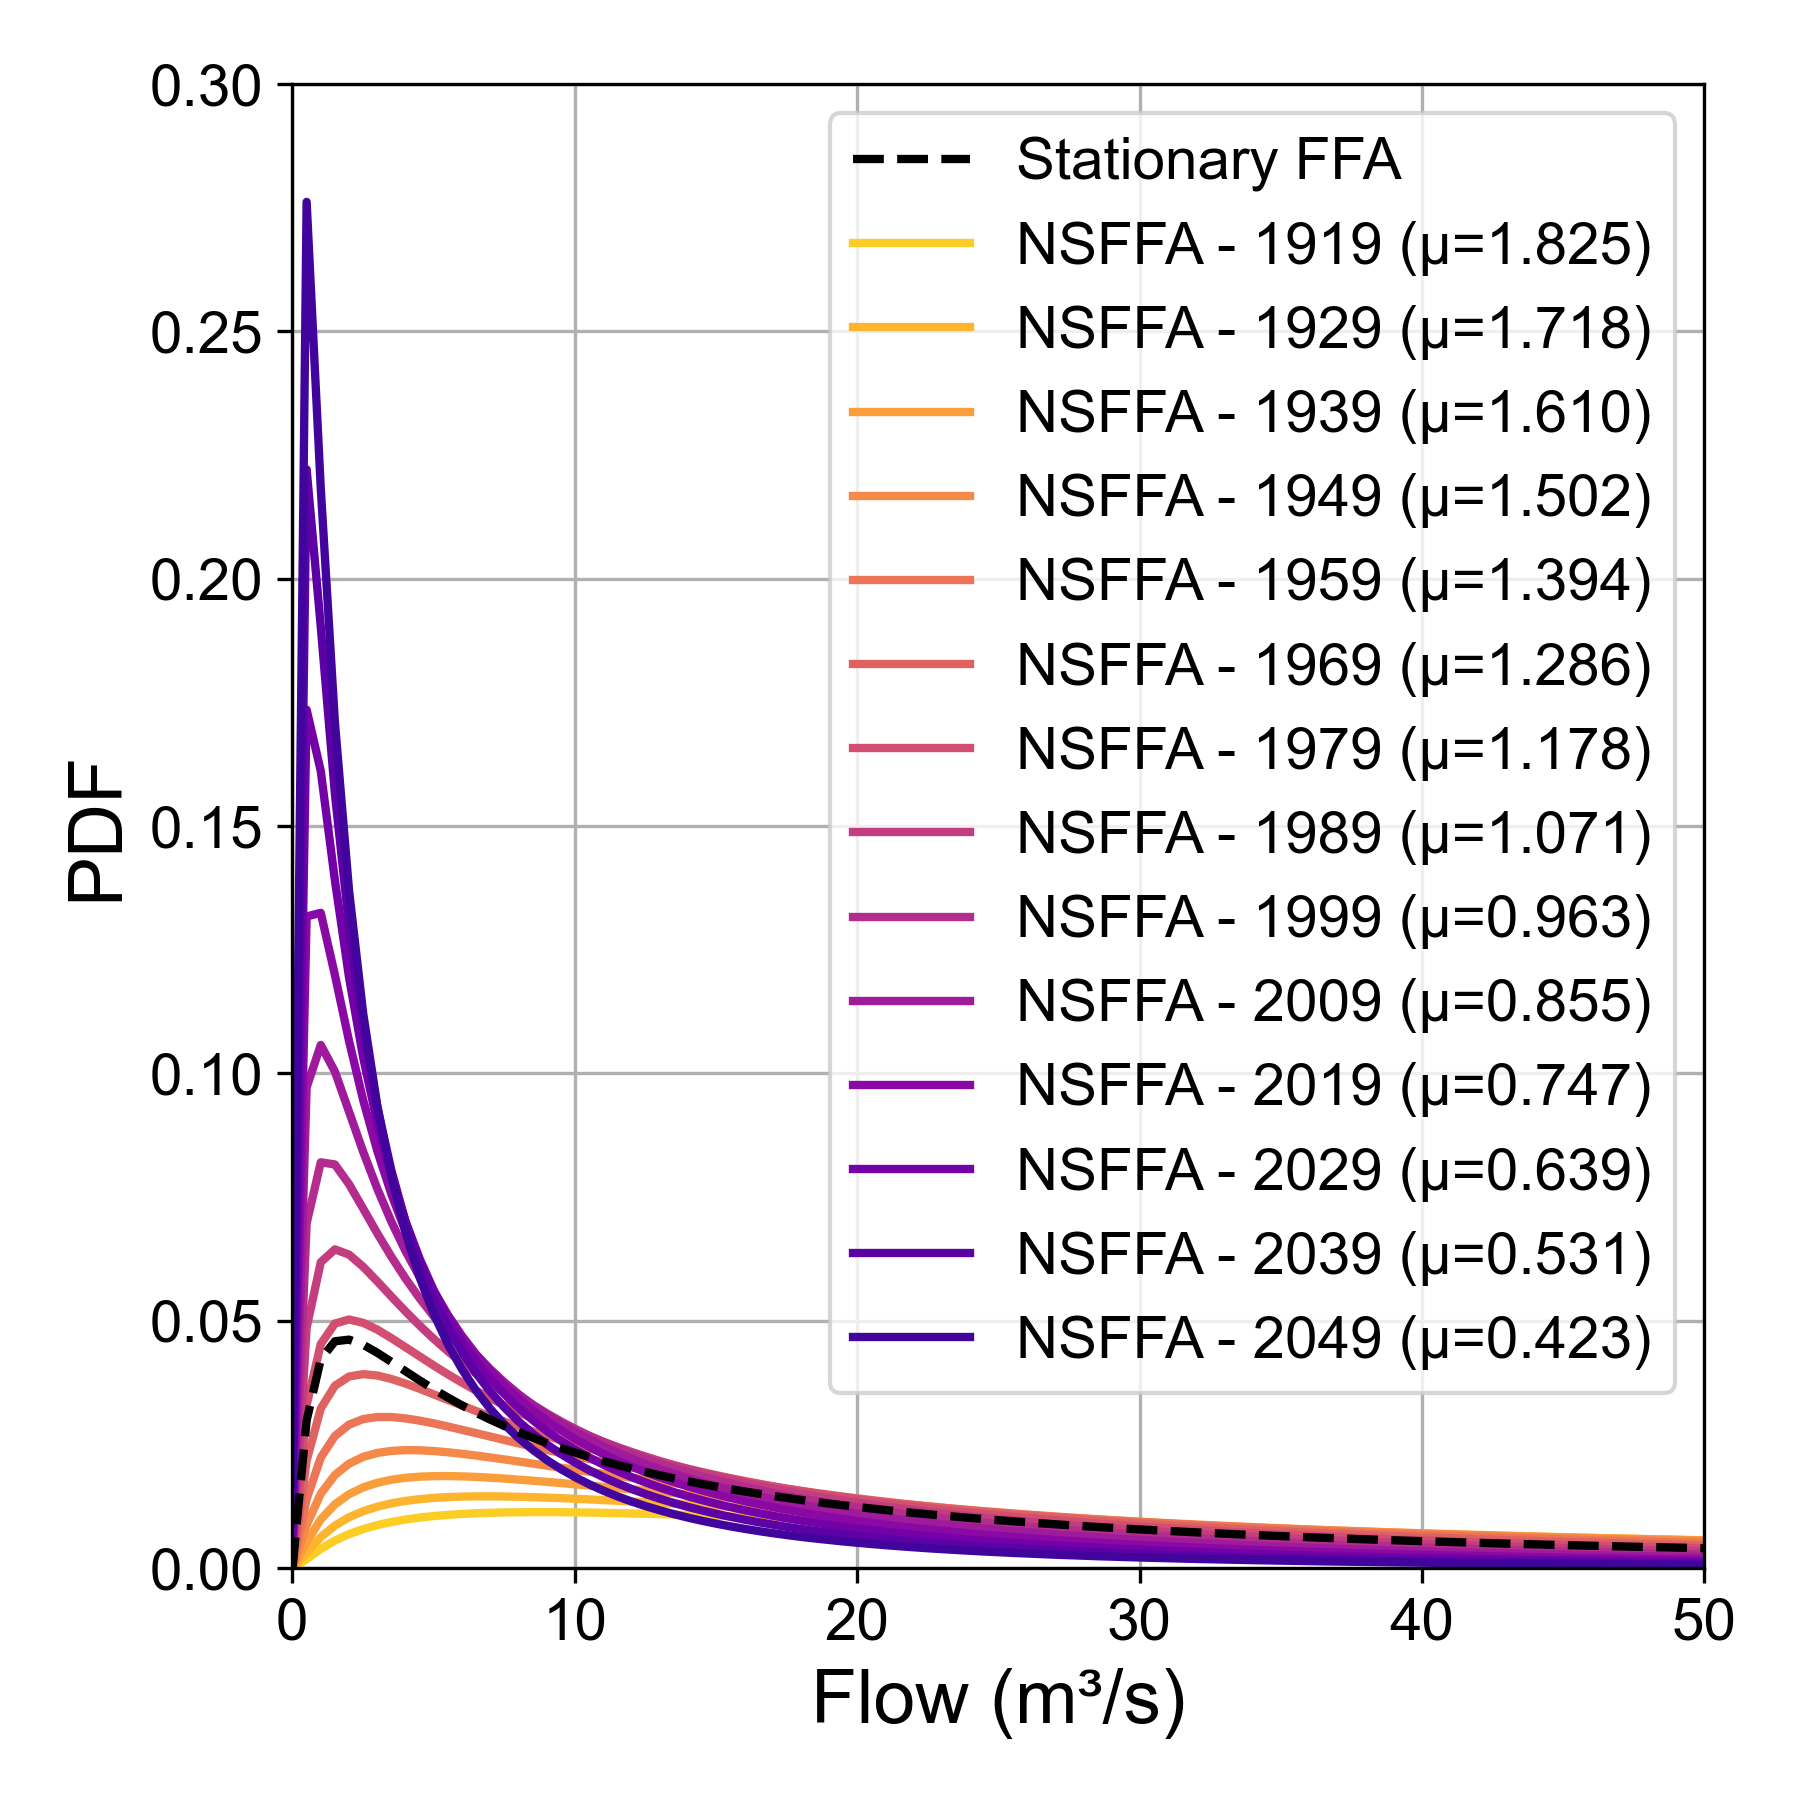
\includegraphics[width=1\linewidth]{_plots/OCD_LP3_linear_mu_comparison_TI.png}
    \caption{Impact of time index selection on posterior mode LP3 distributions under the linear trend NSFFA model for the Fisher Dam dataset.}
    \label{fig:OCD_LP3_linear_mu_comparison_TI}
\end{figure}

\begin{figure*}[ht!]
    \centering
    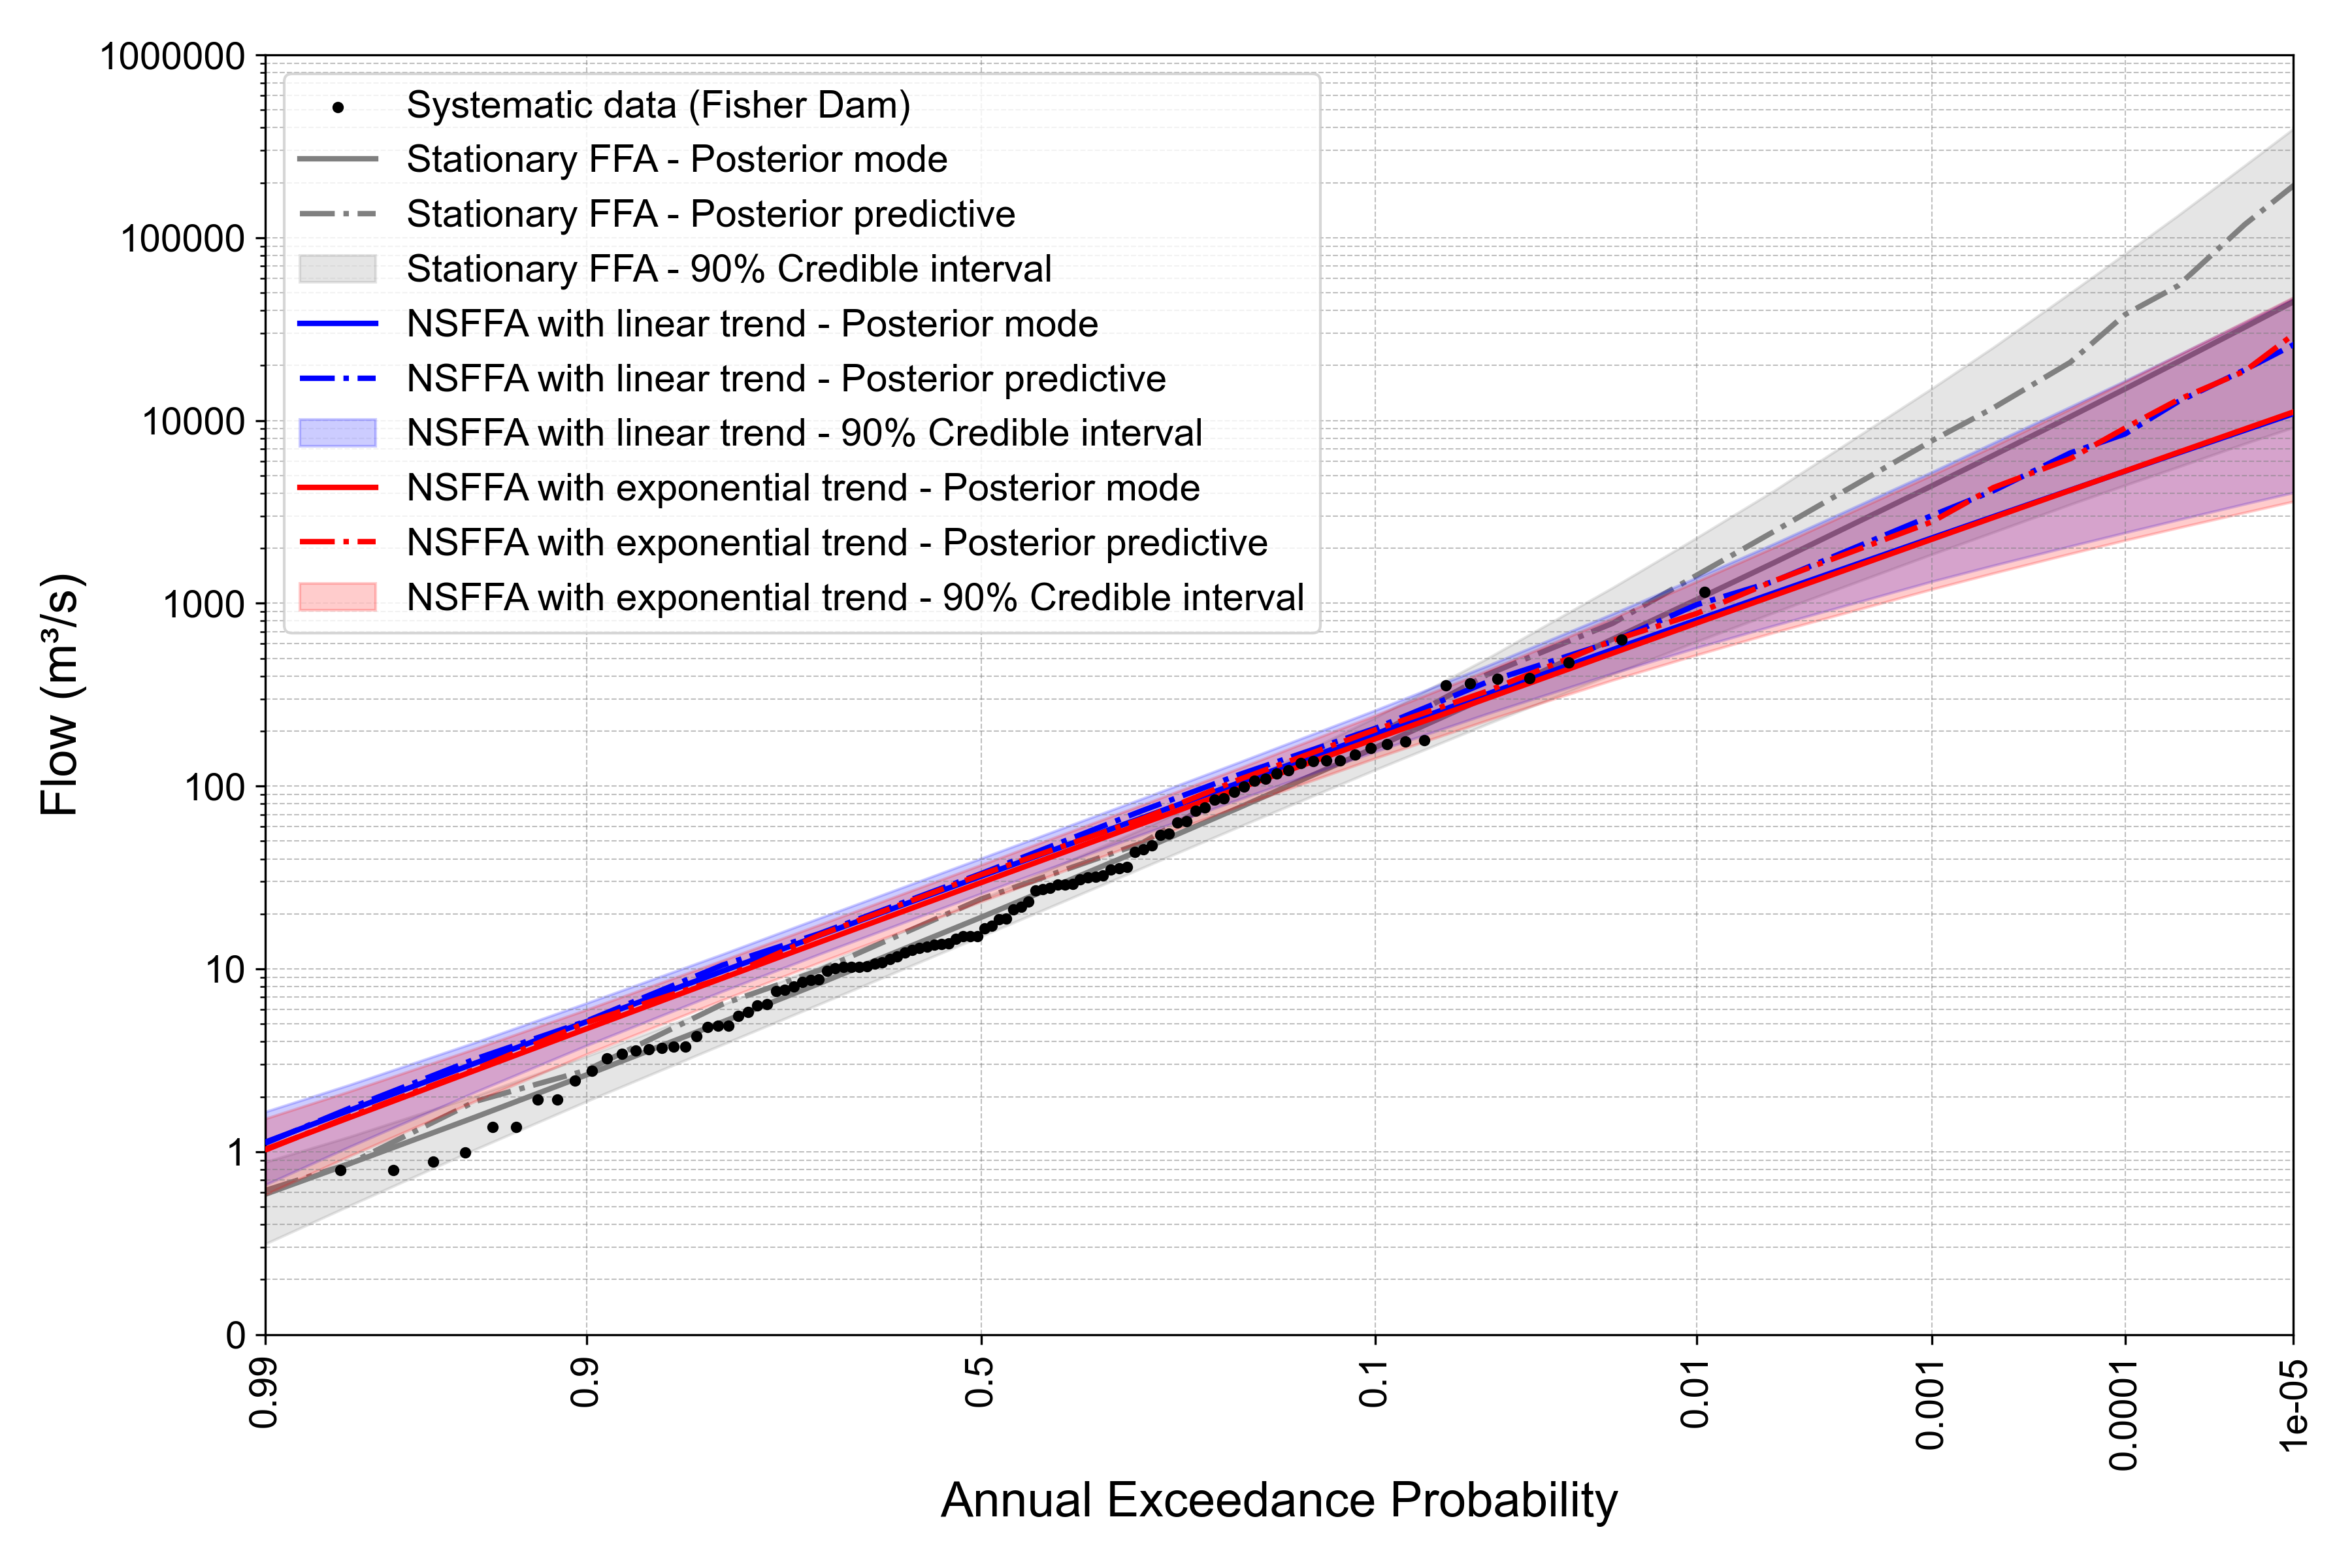
\includegraphics[width=1\linewidth]{_plots/OCD_bayesian_flood_quantiles_lp3_nonstationary.png}    
    \caption{Flood frequency curves derived from stationary FFA and NSFFA models (TI = 1949) compared against observed data for the Fisher Dam dataset. }

    \label{fig:OCD_bayesian_flood_quantiles_lp3_nonstationary}
\end{figure*}

\begin{figure*}[ht!]
    \centering
    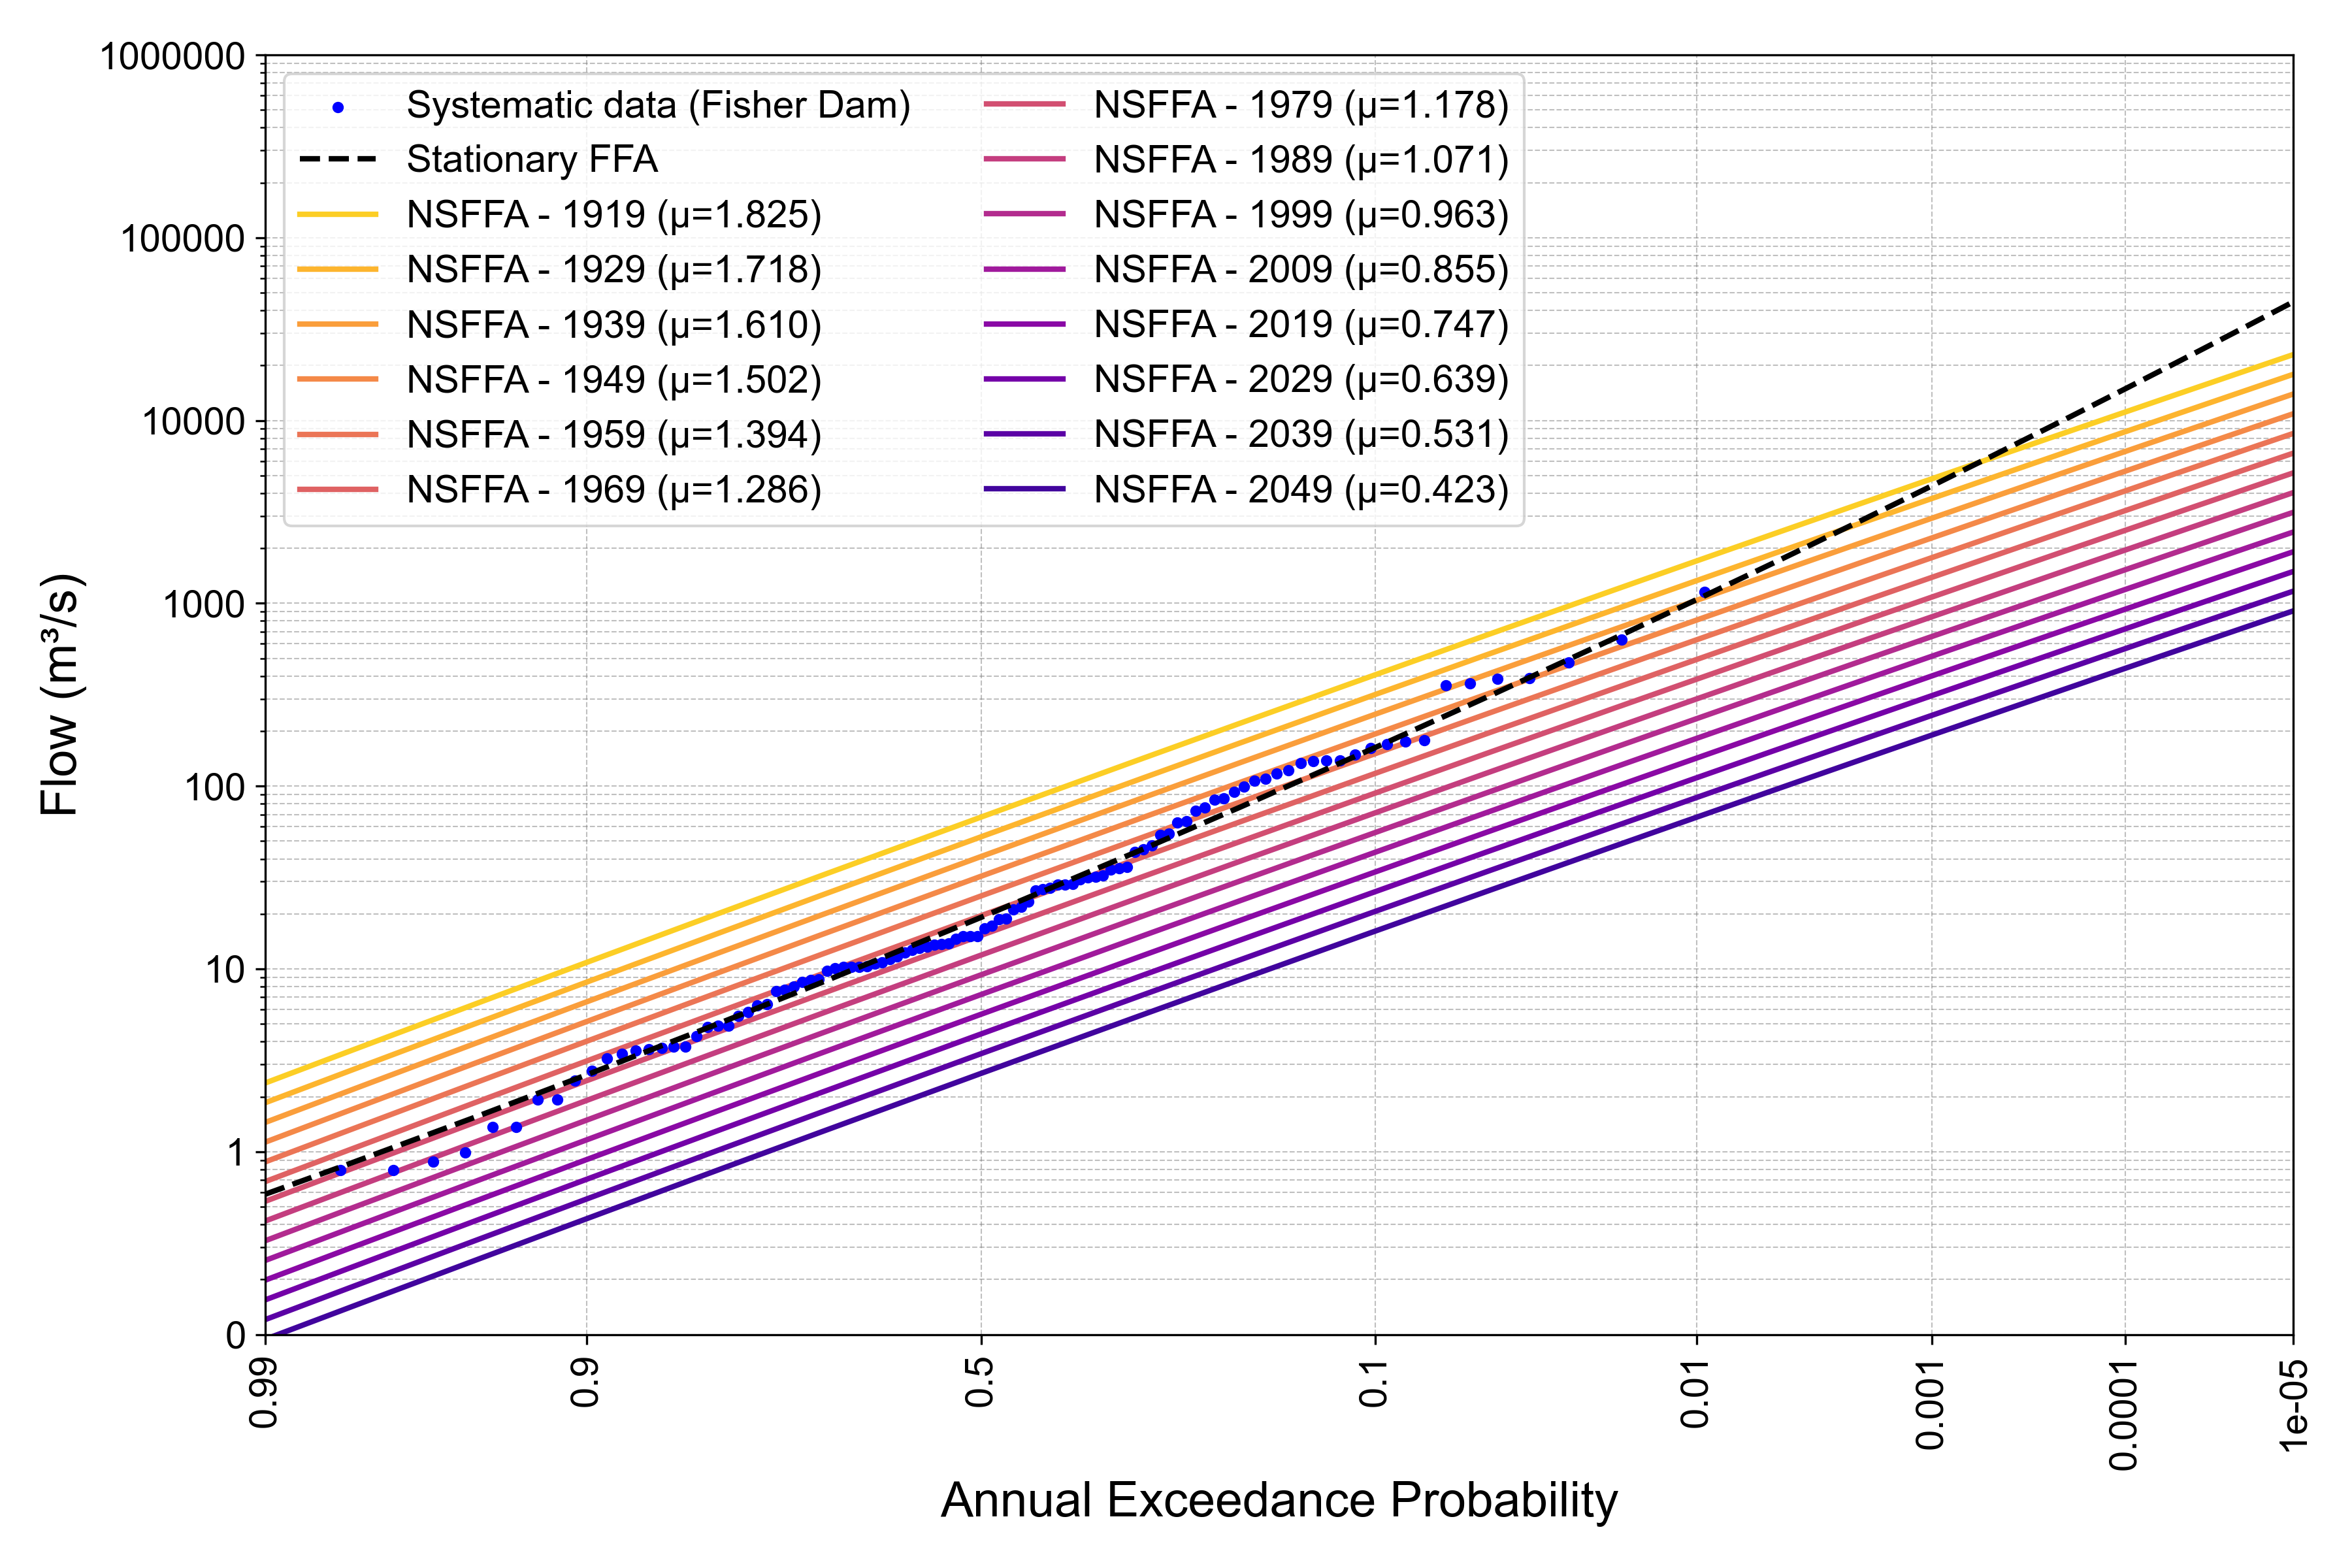
\includegraphics[width=1\linewidth]{_plots/OCD_bayesian_flood_quantiles_lp3_linear_mu_TI.png}
    \caption{Impact of time index selection on flood frequency curves derived from the linear trend NSFFA model compared against stationary FFA and observed data for the Fisher Dam dataset.}
    \label{fig:OCD_bayesian_flood_quantiles_lp3_linear_mu_TI}
\end{figure*}
